\PassOptionsToPackage{unicode=true}{hyperref} % options for packages loaded elsewhere
\PassOptionsToPackage{hyphens}{url}
%
\documentclass[12pt,italian,]{report}
\usepackage{lmodern}
\usepackage{amssymb,amsmath}
\usepackage{ifxetex,ifluatex}
\usepackage{fixltx2e} % provides \textsubscript
\ifnum 0\ifxetex 1\fi\ifluatex 1\fi=0 % if pdftex
  \usepackage[T1]{fontenc}
  \usepackage[utf8]{inputenc}
  \usepackage{textcomp} % provides euro and other symbols
\else % if luatex or xelatex
  \usepackage{unicode-math}
  \defaultfontfeatures{Ligatures=TeX,Scale=MatchLowercase}
\fi
% use upquote if available, for straight quotes in verbatim environments
\IfFileExists{upquote.sty}{\usepackage{upquote}}{}
% use microtype if available
\IfFileExists{microtype.sty}{%
\usepackage[]{microtype}
\UseMicrotypeSet[protrusion]{basicmath} % disable protrusion for tt fonts
}{}
\IfFileExists{parskip.sty}{%
\usepackage{parskip}
}{% else
\setlength{\parindent}{0pt}
\setlength{\parskip}{6pt plus 2pt minus 1pt}
}
\usepackage{hyperref}
\hypersetup{
            pdftitle={Progetto Usabilità e User Experience 2018/2019},
            pdfauthor={Filippo Bartolini; Adamo Fapohunda; Giacomo Leidi; Cristian Castiglione},
            pdfborder={0 0 0},
            breaklinks=true}
\urlstyle{same}  % don't use monospace font for urls
\usepackage{longtable,booktabs}
% Fix footnotes in tables (requires footnote package)
\IfFileExists{footnote.sty}{\usepackage{footnote}\makesavenoteenv{longtable}}{}
\usepackage{graphicx,grffile}
\makeatletter
\def\maxwidth{\ifdim\Gin@nat@width>\linewidth\linewidth\else\Gin@nat@width\fi}
\def\maxheight{\ifdim\Gin@nat@height>\textheight\textheight\else\Gin@nat@height\fi}
\makeatother
% Scale images if necessary, so that they will not overflow the page
% margins by default, and it is still possible to overwrite the defaults
% using explicit options in \includegraphics[width, height, ...]{}
\setkeys{Gin}{width=\maxwidth,height=\maxheight,keepaspectratio}
\setlength{\emergencystretch}{3em}  % prevent overfull lines
\providecommand{\tightlist}{%
  \setlength{\itemsep}{0pt}\setlength{\parskip}{0pt}}
\setcounter{secnumdepth}{0}
% Redefines (sub)paragraphs to behave more like sections
\ifx\paragraph\undefined\else
\let\oldparagraph\paragraph
\renewcommand{\paragraph}[1]{\oldparagraph{#1}\mbox{}}
\fi
\ifx\subparagraph\undefined\else
\let\oldsubparagraph\subparagraph
\renewcommand{\subparagraph}[1]{\oldsubparagraph{#1}\mbox{}}
\fi

% set default figure placement to htbp
\makeatletter
\def\fps@figure{htbp}
\makeatother

\ifnum 0\ifxetex 1\fi\ifluatex 1\fi=0 % if pdftex
  \usepackage[shorthands=off,main=italian]{babel}
\else
  % load polyglossia as late as possible as it *could* call bidi if RTL lang (e.g. Hebrew or Arabic)
  \usepackage{polyglossia}
  \setmainlanguage[]{italian}
\fi

\title{Progetto Usabilità e User Experience 2018/2019}
\author{Filippo Bartolini \and Adamo Fapohunda \and Giacomo Leidi \and Cristian Castiglione}
\date{}

\begin{document}
\maketitle
\begin{abstract}
To Do
\end{abstract}

{
\setcounter{tocdepth}{2}
\tableofcontents
}
\hypertarget{introduzione}{%
\chapter{Introduzione}\label{introduzione}}

Kids Experience è un applicativo web legato al sito madre Kiabi
\url{https://www.kiabi.it/}.

Kiabi è un'azienda francese di e-commerce e distribuzione di
abbigliamento pronto moda, facente parte del gruppo Mulliez. Il suo
slogan \emph{``La moda a piccoli prezzi''} si basa su prodotti a prezzi
accessibili per tutta la famiglia.

Kids Experience offre ai clienti la possibilità di personalizzare
autonomamente megliette per bambini e ragazzi, da 0 a 14 anni, andando
ad ampliare la vasta gamma di prodotti offerti da Kiabi.

L'idea di base e il punto di forza di questa nuova categoria di prodotti
è l'estrema personalizzazione del capo d'abbigliamento scelto da parte
dell'utente.

\hypertarget{ricerca-etnografica}{%
\chapter{Ricerca etnografica}\label{ricerca-etnografica}}

È possibile subito osservare come i bisogni che Kids Experience andrà a
soddisfare non si trovino nei primi livelli della gerarchia di Maslow,
ma si identifichino nel livello intermedio della gerarchia: il livello
di \emph{appartenenza}.

Successivamente si è fatta un'analisi del mercato dell'abbigliamento,
analizzando alcuni competitors attraverso dati reperiti online.
Precisamente, come si evince dalla Fig. 1, per quanto riguarda il
mercato italiano il maggiore esponente è risultato Zara, mentre Kiabi si
posiziona al terzo posto.

\begin{figure}[h]
\centering
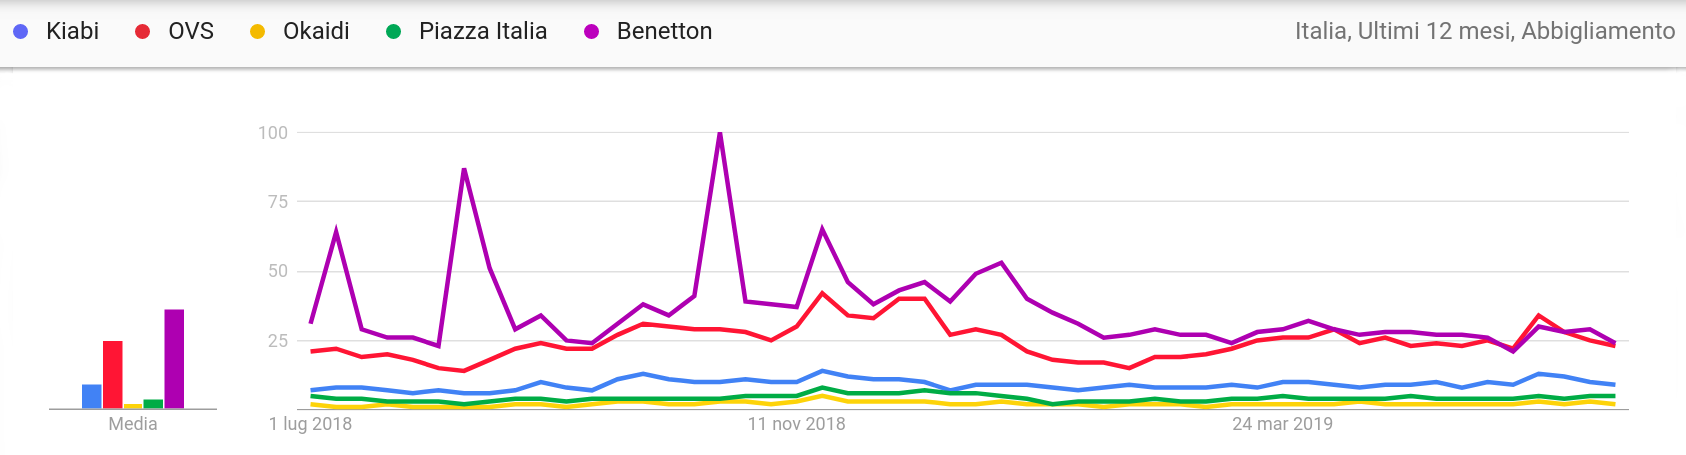
\includegraphics{img/abbigliamento_generico.png}
\caption{Ricerca di mercato abbigliamento}
\end{figure}

Come previsto nell'abbigliamento da bambino Kiabi ha un netto
peggioramento passando dal terzo al quarto posto.

\begin{figure}[h]
\centering
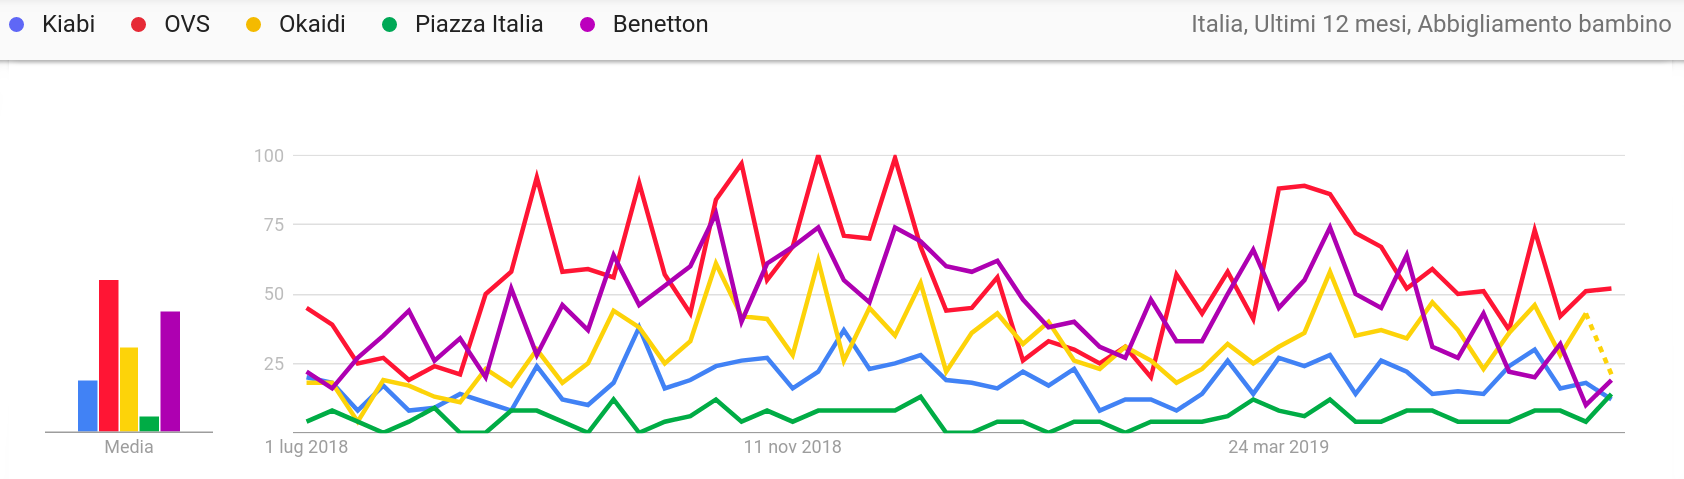
\includegraphics{img/abbigliamento_bambino.png}
\caption{Ricerca di mercato abbigliamento}
\end{figure}

Dopo un'attenta analisi abbiamo deciso di prendere Kiabi, come azienda
madre con l'obiettivo di rilanciarla sul mercato dell'abbigliamento
bambina/o, tramite l'aggiunta di nuove features da noi ideate e proposte
al PM Mulliez.

L'idea di progettare magliette estremamente perzonalizzabili solo per
bambini, nasce dalla semplicità del capo dati i minimi vincoli fisici
(i.e.~taglia) del target. Questo permette di garantire all'utente
un'ampia gamma di personalizzazioni senza dover complicare inutilmente
il processo di manifattura.

\hypertarget{segmentazione}{%
\section{Segmentazione}\label{segmentazione}}

La categoria di utenti principali individuata sono:

\begin{itemize}
\item
  \textbf{Persone di età compresa tra i 30 e i 45 anni}

  Kids Experience è stato concepito prendendo come utenti di riferimento
  adulti di entrambi i sessi e di età compresa tra i 30 e i 45 anni. Si
  suppone che gli utenti abbiano una competenza tecnica e di dominio
  media:

  \begin{itemize}
  \tightlist
  \item
    Capacità di utilizzare un browser
  \item
    Capacità di effettuare acquisti su un e-commerce
  \end{itemize}
\item
  \textbf{Stipendio medio}

  Gli utenti di riferimento hanno un reddito annuo di fascia 20k - 30k:
  leggermente più alto rispetto al reddito annuo medio italiano delle
  regioni del centro nord ((«Il sole 24 ore: stipendi d'Italia»,
  \protect\hyperlink{ref-redditomedio}{s.d.})).
\item
  \textbf{Nazionalità}

  Italiana
\end{itemize}

Si considerano come utenti secondari:

\begin{itemize}
\item
  \textbf{Adulti}

  Tendenzialmente legati agli utenti principali, con compentenze
  tecniche e di dominio nella media:

  \begin{itemize}
  \tightlist
  \item
    Capacità di utilizzare un browser
  \item
    Capacità di effettuare acquisti su un e-commerce
  \end{itemize}
\end{itemize}

\hypertarget{user-research}{%
\section{User research}\label{user-research}}

Per avere un'idea sui comportamenti degli utilizzatori principali del
sito, ossia le coppie, è stata fatta una ricerca tra le varie indagini
di mercato disponibili sul web.
\\
Prendendo in esame \href{http://siqual.istat.it/SIQual/visualizza.do?id=0021002\&refresh=true\&language=IT}{l'indagine}
svolta dall'Istituto Nazionale di Statistica (ISTAT), si può notare come la spesa media italiana familiare mensile per l'abbigliamento sia di 83.89€.

In particolare, ripartita come segue, sulla base del reddito familiare:

\begin{figure}[h]
\centering
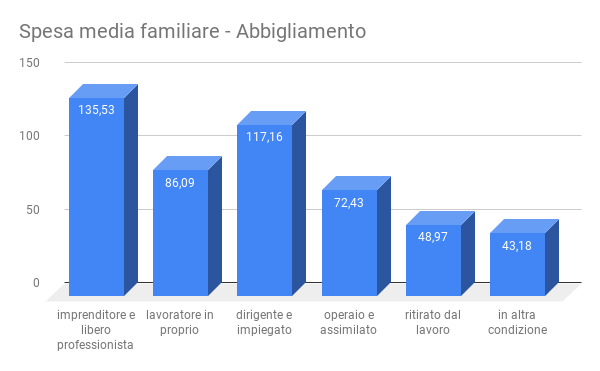
\includegraphics[width=0.7\textwidth,height=\textheight]{img/Spesa_media_familiare_abbigliamento.png}
\caption{Spesa media familiare per l'abbigliamento}
\end{figure}

Estraendo i soli dati riguardanti le famiglie con figli, otteniamo il
seguente grafico:

\begin{figure}[h]
\centering
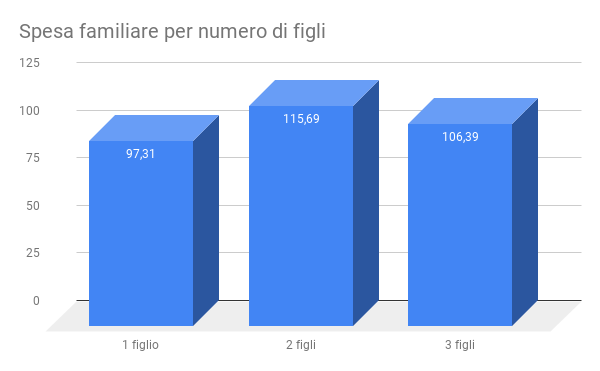
\includegraphics[width=0.7\textwidth,height=\textheight]{img/Spesa_familiare_per_numero_di_figli.png}
\caption{Spesa media familiare per numero di figli}
\end{figure}

dal quale si evince che, per quanto riguarda l'abbigliamento, la spesa
più alta è sostenuta dalle famiglie con 2 figli.

\hypertarget{valutazione-delle-risorse-esistenti}{%
\chapter{Valutazione delle risorse
esistenti}\label{valutazione-delle-risorse-esistenti}}

Prendiamo in considerazione diversi siti web di concorrenti che a
differenza di Kiabi sono focalizzati esclusivamente sulla
personalizzazione delle magliette e che operano a livello nazionale e
internazionale.

I siti presi in considerazione sono i seguenti: ERR

\begin{itemize}
\tightlist
\item eshirt
\item H\&M
\item Kiabi
\end{itemize}

\hypertarget{expert-usability-review}{%
\section{Expert Usability Review}\label{expert-usability-review}}

L'analisi effettuata in questa fase è avvenuta adottando le linee guida
``le 10 euristiche di Nielsen e Molich'' e a tali euristiche sono state
affiancate alcune delle euristiche di Weinshenk e Barker:

\begin{enumerate}
\def\labelenumi{\arabic{enumi}.}
\item
  \textbf{Visibilità dello stato del sistema}

  Il sistema dovrebbe tenere sempre l'utente informato su cosa succede
  nel sistema attraverso l'uso di feedback appropriati forniti in tempi
  ragionevoli.
\item
  \textbf{Corrispondenza tra sistema e mondo reale}

  Il sistema dovrebbe ``parlare'' la lingua dell'utente con parole,
  frasi e concetti familiari all'utente invece che utilizzare termini
  propri del sistema.
\item
  \textbf{Controllo e libertà}

  Dato che l'utente spesso usa delle funzionalità del sistema per
  errore, è sempre necessario fornire un modo per uscire dallo stato in
  cui si è venuto a trovare.
\item
  \textbf{Consistenza e standard}

  Utenti non dovrebbe avere dubbi riguardo al fatto che parole,
  situazioni, azioni differenti abbiano lo stesso effetto.
\item
  \textbf{Prevenzione dell'errore}

  Il miglior modo per evitare un errore, è prevenirlo.
\item
  \textbf{Riconoscimento anziché ricordo}

  Minimizzare il carico cognitivo dell'utente rendendo gli oggetti, le
  azioni e le opzioni più visibili possibili. Gli utenti non dovrebbero
  ricordare le informazioni da un dialogo all'altro.
\item
  \textbf{Flessibilità ed efficienza d'uso}

  Il sistema deve facilitare l'uso anche agli utenti esperti,
  permettendogli di personalizzare le azioni più frequenti.
\item
  \textbf{Design ed estetica minimalista}

  I dialoghi non dovrebbero contenere informazioni che sono irrelevanti
  o di cui si ha raramente bisogno. Ogni informazione extra compete con
  le informazioni rilevanti e diminuisce la loro visibilità.
\item
  \textbf{Aiuto all'utente}

  Gli errori dovrebbero essere mostrati in un linguaggio chiaro,
  indicando in modo preciso il problema e suggerendo la soluzione.
\item
  \textbf{Documentazione}
\end{enumerate}

Sarebbe meglio fornire un'adeguata documentazione, a presciendere dal
fatto che il sito potrebbe essere utilizzato anche senza. Questo genere
di informazione dovrebbe essere facile da cercare, focalizzata sul task
dell'utente e dovrebbe elencare una sequenza di passi semplici da
completare.

\begin{enumerate}
\def\labelenumi{\arabic{enumi}.}
\setcounter{enumi}{10}
\tightlist
\item
  \textbf{Predicibilità}
\end{enumerate}

L'utente sarà in grado di costruire un modello mentale di come il
sistema risponderà alle sue azioni.

\begin{enumerate}
\def\labelenumi{\arabic{enumi}.}
\setcounter{enumi}{11}
\tightlist
\item
  \textbf{Limitazioni umane}
\end{enumerate}

Il design deve tener conto delle limitazioni cognitive e sensoriali per
evitare un sovraccarico cognitivo.

\begin{enumerate}
\def\labelenumi{\arabic{enumi}.}
\setcounter{enumi}{12}
\tightlist
\item
  \textbf{Precisione}
\end{enumerate}

L'interfaccia permette all'utente di portare a termine il task con
esattezza

\hypertarget{ispezione-eshirt-eshirt}{%
\subsection{\texorpdfstring{Ispezione Eshirt («Eshirt»,
\protect\hyperlink{ref-eshirt}{s.d.})}{Ispezione Eshirt («Eshirt», s.d.)}}\label{ispezione-eshirt-eshirt}}

\hypertarget{prima-ispezione}{%
\subsubsection{Prima ispezione}\label{prima-ispezione}}

Il sito www.eshirt.it si presenta con una schermata iniziale ben
organizzata in cui è possibile scegliere il capo d'abbigliamento da
personalizzare, tra uomo, donna, bambino o un gadget/accessorio.
Successivamente, tramite altre tre pagine, si potrà scegliere nello
specifico, la tipologia del capo d'abbigliamento o del gadget, le sue
caratteristiche principali ed infine la quantità. La quarta pagina è
quella che offre la vera e propria interfaccia di personalizzazione del
prodotto precedentemente scelto, mentre la quinta ed ultima pagina offre
la possibilità di scegliere la taglia (``unica'' nel caso dei gadget) e
di aggiungere il prodotto al carrello.

Dalla pagina principale si può, inoltre, accedere a due sezioni ``idee''
e ``disegni'' in cui vengono mostrati dei prototipi di capi già
personalizzati per diversi eventi e occasioni. Purtroppo la maggior
parte dei prodotti vengono mostrati uguali e identici in entrambe le
sezioni.

Fin da subito si nota che il numero di scelte in ogni pagina è piuttosto
esiguo (per essere un sito che offre il servizio di personalizzazione) e
in alcun modo ampliabile. In particolare, sia la personalizzazione del
capo d'abbigliamento che quella del gadget consiste solamente nella
scelta del colore e nell'aggiunta di un testo e/o di un'immagine. Questi
elementi di personalizzazione seguono i principi di Gestalt: sono
chiari, estremamente semplici e intuitivi nel loro utilizzo.

Durante la personalizzazione del proprio prodotto c'è anche la
possibilità di condividerlo sui social o di inviarlo tramite
mail/messaggio. Il colore del font utilizzato in alcune pagine del sito
è piuttosto chiaro e in alcuni casi di difficile lettura, mentre la
dimensione del font risulta appropriata. Le informazioni sono scritte
utilizzando un linguaggio semplice che ne rendono chiaro il contenuto.
Non c'è nessuna differenza nell'utilizzo dell'intero sistema da parte di
un utente esperto o di un novizio: non sono presenti né shortcut né
metodi di personalizzazione avanzati. Non esiste un sistema di
registrazione per discriminare un utente da un altro.

L'impressione che ne deriva è tutto sommata positiva, nonostante la
parte di personalizzazione sia da rivedere in quanto è troppo limitata.

\hypertarget{analisi-diretta-sistema---linee-guida}{%
\subsubsection{Analisi diretta: Sistema - Linee
guida}\label{analisi-diretta-sistema---linee-guida}}

Effettuando un'analisi diretta sono stati riscontrati una serie di
problemi dovuti alla violazione delle euristiche di Nielsen e delle
ulteriori euristiche definite durante l'ispezione.

Le euristiche non rispettate individuate sono le seguenti:

\begin{itemize}
\item
  Lo stato del sistema non è visibile durante le operazioni di aggiunta
  del testo o di caricamento di una immagine. Inoltre, non è possibile
  capire qual è lo stato di avanzamento di un ordine (non c'è una barra
  che mostri lo stato di avanzamento della personalizzazione). Non
  rispetta l'euristica della \emph{visibilità dello stato del sistema}.
\item
  Quando si inserisce del testo, l'utente viene portato in una schermata
  con un editor testuale dalla quale non è possibile continuare a
  visualizzare le modifiche già fatte. L'unico elemento grafico di
  riconoscimento della piattaforma rimane il logo in alto. Non rispetta
  l'euristica della \emph{consistenza e standard}.
\item
  Non esiste una caratterizzazione dell'utenza in base alla conoscenza
  del dominio applicativo. Non rispetta l'euristica della
  \emph{flessibilità d'uso}.
\item
  Ogniqualvolta si torna indietro dalla schermata di modifica, un modale
  blocca il flusso di esecuzione. Non rispetta l'euristica di
  \emph{design ed estetica minimalista}.
\item
  L'interfaccia presenta dei ritardi che rendono difficile l'esecuzione
  dei task con precisione. Non rispetta l'euristica \emph{Precisione}.
\end{itemize}

\hypertarget{analisi-inversa-linee-guida---sistema}{%
\subsubsection{Analisi inversa: Linee guida -
Sistema}\label{analisi-inversa-linee-guida---sistema}}

Con l'analisi inversa vengono confrontate le linee guida con il sistema,
utilizzando le euristiche sopradescritte e mettendo in evidenza quelle
che non vengono rispettate.

\begin{enumerate}
\def\labelenumi{\arabic{enumi}.}
\tightlist
\item
  \textbf{Visibilità dello stato del sistema}: il sistema non fornisce
  feedback sullo stato di avanzamento durante l'aggiunta di una modifica
\item
  \textbf{Corrispondenza tra sistema e mondo reale}: euristica
  rispettata
\item
  \textbf{Controllo e libertà}: euristica rispettata
\item
  \textbf{Consistenza e standard}: l'interfaccia non è consistente in
  quanto bottoni della stessa categoria (i.e.~inserimento di testo e
  inserimento di immagini) hanno comportamenti diversi
\item
  \textbf{Prevenzione dell'errore}: euristica rispettata
\item
  \textbf{Riconoscimento anziché ricordo}: euristica rispettata
\item
  \textbf{Flessibilità d'uso}: vedi analisi diretta
\item
  \textbf{Design ed estetica minimalista}: alcuni modali contengono
  informazioni inutili ai fini del processo di personalizzazione
\item
  \textbf{Aiuto all'utente}: euristica rispettata
\item
  \textbf{Documentazione}: inesistente
\item
  \textbf{Predicibilità}: euristica rispettata
\item
  \textbf{Limitazioni umane}: euristica rispettata
\item
  \textbf{Precisione}: vedi analisi diretta
\end{enumerate}

\hypertarget{ispezione-brosprint-brosprint}{%
\subsection{\texorpdfstring{Ispezione Brosprint
({\textbf{???}})}{Ispezione Brosprint (???)}}\label{ispezione-brosprint-brosprint}}

\hypertarget{prima-ispezione-1}{%
\subsubsection{Prima ispezione}\label{prima-ispezione-1}}

La home del sito si presenta minimale e pulita. Viene data molta
importanza all'header che contiene un carusel che mostra le offerte
principali oltre al logo dell'azienda. Con uno scroll verso il basso è
possibile accedere alla vera e propria home. Vengono subito esposte
quattro categorie con foto esemplificative: Uomo, donna, bambino e
gadget. Ogni categoria viene articolata in sotto categorie che indicano
il capo specifico che si vuole personalizzare. Es: sotto uomo troviamo:
T-shirt, polo felpe, camicia, canotta, pantaloni e pile. Per quanto
riguarda la categoria ``bambino'' la scelta è leggermente più limitata,
offre: T-shirt, polo, felpe e linea baby (la linea studiata
appositamente per i bambini).

Con un ulteriore scroll in basso viene mostrata la sezione ``Cosa
Facciamo'' con descrizione dei tipi di stampa disponibile. A seguire
``Cosa puoi personalizzare con noi'' dove viene passato in rassegna il
catalogo dei capi personalizzabili.

Infine scrollando ancora vi è la sezione con i link alle informazioni di
carattere generale (spedizione, metodo di pagamento, partner e
fornitori) e le FAQ.

L'esperienza di acquisto è semplice, lineare e sono sufficienti pochi
click per portare a termine l'acquisto. Selezionando una categoria si
viene reindirizzati ad una pagina dove l'utente può selezionare il tipo
di capo, che fa da filtro per le sezioni successive, rendendo possibile
visualizzare solo i capi di interesse (es: magliette a maniche corte).

Scrollando verso il basso (funzionalità ben segnalata da una freccia)
vengono mostrati uno dopo l'altro i capi specifici.

Di ogni capo è possibile selezionare taglia e colore.

Per ogni capo mostrato vengono messi due bottoni molto grandi e visibili
che espongono due funzioni: ``Dettagli'' e ``Preventivo'', la prima
permette all'utente di visualizzare informazioni come grammatura del
capo, tessuto, tipo di rifiniture, ecc. Mentre la seconda serve a
concludere effettivamente l'ordine.

Una serie di menù dropdown permettono di selezionare la taglia e il
colore desiderato in base a quelli disponibili e i punti dove è
possibile effettuare le stampe.

Inoltre nella parte alta di ogni pagina relativa all'acquisto viene
mostrato un banner che recita ``Hai problemi a concludere la
personalizzazione? Contattaci via email o in chat'' che offre la
possibilità di farsi assistere durante la fase di personalizzazione.

\hypertarget{analisi-diretta-sistema---linee-guida-1}{%
\subsubsection{Analisi diretta: Sistema - linee
guida}\label{analisi-diretta-sistema---linee-guida-1}}

Effettuando un'analisi diretta sono stati riscontrati una serie di
problemi dovuti alla violazione delle euristiche di Nielsen e delle
ulteriori euristiche definite durante l'ispezione.

Le euristiche non rispettate individuate sono le seguenti:

\begin{itemize}
\item
  Non rispetta l'euristica riguardante lo \emph{stato del sistema} in
  quanto entrando nella pagina di personalizzazione non è deducibile lo
  stato di avanzamento della personalizzazione.
\item
  Le operazioni di annullamento e ripristino dello stato precedente sono
  macchinose in quanto l'interfaccia è composta da una lunga serie di
  menù a tendina, contraddicendo l'euristica di \emph{controllo e
  libertà} e \emph{prevenzione dell'errore}.
\item
  Gli stessi bottoni su pagine diverse hanno comportamenti diversi. Non
  rispetta l'euristica di \emph{consistenza e standard}
\item
  Non rispetta l'euristica \emph{riconoscimento anziché ricordo} in
  quanto l'utente è costretto a ricordare tutte le modifiche
  precedentemente selezionate perché non è possibile visualizzarle tutte
  insieme contemporaneamente.
\item
  Non rispetta l'euristica della \emph{flessibilità d'uso} perchè non
  sono presenti shortcut che agevolino l'utente esperto.
\item
  Non rispetta l'euristica della \emph{precisione} perchè il sistema è
  ritenuto ``non preciso'', in quanto alcuni menù non sono cliccabili
  per intero, ciò costrige l'utente a selezionare attentamente l'area in
  cui cliccare.
\end{itemize}

In generale il sistema presenta una minima gamma di personalizzazioni.

\hypertarget{analisi-inversa-linee-guida---sistema-1}{%
\subsubsection{Analisi inversa: Linee guida -
Sistema}\label{analisi-inversa-linee-guida---sistema-1}}

Con l'analisi inversa vengono confrontate le linee guida con il sistema,
utilizzando le euristiche sopradescritte e mettendo in evidenza quelle
che non vengono rispettate.

\begin{enumerate}
\def\labelenumi{\arabic{enumi}.}
\tightlist
\item
  \textbf{Visibilità dello stato del sistema}: il sistema non fornisce
  feedback durante le operazioni di personalizzazione del prodotto
\item
  \textbf{Corrispondenza tra sistema e mondo reale}: euristica
  rispettata
\item
  \textbf{Controllo e libertà}: l'utente non ha alcun controllo
  sull'avanzamento del processo di personalizzazione
\item
  \textbf{Consistenza e standard}: nell'editor di personalizzazione
  bottoni identici si comportano in maniera differente rompendo la
  consistenza del sito
\item
  \textbf{Prevenzione dell'errore}: non esiste un modo per accorgersi di
  eventuali errori nel processo di personalizzazione
\item
  \textbf{Riconoscimento anziché ricordo}: sovraccarico cognitivo dovuto
  alla scarsa capacità dell'interfaccia di organizzare le informazioni
  in modo chiaro
\item
  \textbf{Flessibilità d'uso}: non vengono offerte scorciatoie per gli
  utenti esperti
\item
  \textbf{Design ed estetica minimalista}: euristica rispettata
\item
  \textbf{Aiuto all'utente}: euristica rispettata
\item
  \textbf{Documentazione}: inesistente
\item
  \textbf{Predicibilità}: cfr. euristica 4
\item
  \textbf{Limitazioni umane}: euristica rispettata
\item
  \textbf{Precisione}: i ritardi nell'interfaccia la rendono di
  difficile utilizzo, inoltre alcuni elementi che appaiono cliccabili
  non lo sono completamente
\end{enumerate}

\hypertarget{ispezione-qualcosa}{%
\subsection{Ispezione qualcosa}\label{ispezione-qualcosa}}

\hypertarget{user-testing}{%
\section{User testing}\label{user-testing}}

In seguito alla mancanza di un team specializzato per il testing del
software si è deciso di usare il \emph{discount usability testing}
proposta da Nielsen, nello specifico la metodologia di testing usata è
\emph{Thinking Aloud}.

Sono stati dunque scelti 4 utenti che rispettano il target scelto e ad
ognuno di loro è stato chiesto di portare a termine 4 task per poter
osservare gli errori e i punti critici del sistema.

\hypertarget{protocollo-di-testing}{%
\subsection{Protocollo di testing}\label{protocollo-di-testing}}

\begin{itemize}
\item
  \textbf{Tipologia}: Discount usability testing
\item
  \textbf{Metodologia}: Thinking Aloud
\item
  \textbf{Task da testare}: ERR task specifici per il sito preso in
  considerazione

  \begin{enumerate}
  \def\labelenumi{\arabic{enumi}.}
  \tightlist
  \item
    Modificare un progetto personale
  \item
    Condividere sui social un progetto
  \item
    Aggiungere dettagli al collo di una maglietta
  \item
    Votare un progetto presente nel catalogo
  \end{enumerate}
\item
  \textbf{Descrizione dei risultati}:

  \begin{itemize}
  \item
    \textbf{Sfumature sul compimento del task}: necessità di
    suggerimenti da parte degli osservatori
  \item
    \textbf{Errori}:

    \begin{itemize}
    \tightlist
    \item
      Catastrofici: fallimento del task
    \item
      Gravi: rallentamento notevole nell'esecuzione del task
    \item
      Minori: rallentamento sensibile nell'esecuzione del task
    \item
      Cosmetici: fastidio all'utente senza rallentamento visibile
      nell'esecuzione del task
    \end{itemize}
  \end{itemize}
\item
  \textbf{Domande post-sessione}:

  \begin{itemize}
  \tightlist
  \item
    System Usability Scale (SUS)
  \end{itemize}
\item
  \textbf{Scelta dei soggetti}: effettuata di comune accordo con i
  membri del team
\item
  \textbf{Organizzazione del test}: test condotti in presenza del team
\end{itemize}

\hypertarget{risultati-test}{%
\subsection{Risultati test}\label{risultati-test}}

Ad ogni utente sono stati proposti i quattro task sopracitati da
realizzare sul sito, quattro compiti specifici da portare a termine
utilizzando l'interfaccia dal sito Kids Experience. ERR kids experience?
NO

I task sono stati scritti su carta e presentati all'utente.
L'osservatore si è preoccupato di preparare l'ambiente per lo
svolgimento del test e di spiegare al tester il motivo del testing,
mettendolo a suo agio spiegando che è il sistema ad essere valutato e
non le sue capacità e, in caso cui fosse stato troppo in silenzio o
bloccato su un punto, ha cercato di spingerlo a provare nuovamente senza
fornire alcun aiuto esplicito. Durante il testing l'osservatore ha preso
appunti segnando eventuali problemi incontrati.

Alla fine del test è stato proposto all'utente il questionario SUS così
formato:

\begin{enumerate}
\def\labelenumi{\arabic{enumi}.}
\tightlist
\item
  Penso che userei questo sistema con frequenza
\item
  Ho trovato il sistema troppo complesso
\item
  Penso che il sistema sia facile da usare
\item
  Penso che avrei bisogno dell'aiuto di una persona esperta per essere
  in grado di usare il sistema
\item
  Ritengo che le varie funzionalità di questo sistema siano ben
  integrate
\item
  Ritengo che il sistema sia inconsistente
\item
  Penso che la maggior parte della gente sia in grado di imparare
  velocemente ad usare questo sistema
\item
  Ritengo che il sistema sia poco maneggevole
\item
  Mi sono sentito molto sicuro nell'utilizzo del sistema
\item
  Ho avuto bisogno di imparare molte cose prima di potermi sicuro
  nell'utilizzo del sistema
\end{enumerate}

ERR i risultati dove sono?

\hypertarget{studio-di-fattibilituxe0}{%
\chapter{Studio di fattibilità}\label{studio-di-fattibilituxe0}}

In questa fase verranno analizzati i ``Contesti d'uso'', gli
``Scenarios'' e le ``Personas''.

I ``Contesti d'uso'' descrivono in modo chiaro e preciso le
caratteristiche degli utenti target e dei task che dovranno svolgere e
gli eventuali vincoli presenti.

Gli ``Scenarios'' sono brevi storie che raccontano in dettaglio come
l'utente realizza l'obiettivo personale eseguendo uno o più dei compiti
pianificati sul sistema.

Infine si rappresenteranno le ``Personas'', ovvero verranno descritti,
in modo dettagliato, gli utenti che utilizzeranno il sistema.

\hypertarget{contesto-duso}{%
\section{Contesto d'uso}\label{contesto-duso}}

ERR ?

\hypertarget{vincoli-ambientali}{%
\subsection{Vincoli ambientali}\label{vincoli-ambientali}}

Si presuppone un utilizzo tipico del sito per gli acquisti in un
ambiente tranquillo come quello domestico o simili, dove l'utente si
possa concentrare, se necessario, nella personalizzazione dei prodotti.
Tale ambiente non comporta quindi vincoli particolari.

\hypertarget{vincoli-tecnici}{%
\subsection{Vincoli tecnici}\label{vincoli-tecnici}}

Il sito web richiede una connessione ad Internet per essere utilizzato.
L'interfaccia è progettata, con le tecnologie attuali, in maniera tale
da garantire e supportare una buona esperienza di utilizzo da PC.
Inoltre a causa delle potenzialità di personalizzazione dell'editor,
risulta più comodo l'accesso da dispositivi notebook e desktop.

\hypertarget{scenarios}{%
\section{Scenarios}\label{scenarios}}

\hypertarget{severina-millanta---qualcosa-di-unico-per-la-bambina}{%
\subsection{Severina Millanta - Qualcosa di unico per la
bambina}\label{severina-millanta---qualcosa-di-unico-per-la-bambina}}

Sta per arrivare il compleanno della bambina e Severina ha già
provveduto a organizzare una festa in cui invitare i compagni di scuola
e relativi genitori.

Dopo aver organizzato la festa non resta che pensare al regalo. Parlando
con le altre mamme ha convenuto che la cosa migliore sarebbe comprare un
capo di abbigliamento. Severina però non vuole ripiegare sulle classiche
cose che si possono reperire nei negozi, vuole qualcosa di unico che
parli della sua bambina e che le faccia fare bella figura con le altre
mamme. Inizialmente pesa di recarsi da un sarto, ma dato il costo e il
tempo di attesa capisce subito che non è la scelta vincente.

Inizia a scrivere post spiegando la problematica su un paio di forum.
Tra i vari consigli ne spunta uno che risponde esattamente alle sue
esigenze: facile da usare, altamente personalizzabile e veloce nella
consegna.

\hypertarget{antonio-frastani---una-maglietta-da-campione}{%
\subsection{Antonio Frastani - Una maglietta da
campione}\label{antonio-frastani---una-maglietta-da-campione}}

Da alcuni giorni la sua ragazza non fa altro che raccontare ad Antonio
le avventure del suo primo nipotino. Il bambino, a quanto pare, passa le
giornate al parco a giocare a calcio con gli amici e sogna da grande di
entrare in una squadra professionistica.

Antonio, dopo una lunga giornata di lavoro, decide di fare un regalo al
nipote della sua ragazza. Antonio si mette a cercare su Google un
possibile regalo per un bambino di 7 anni. Su un forum di settore gli
viene consigliata la possibilità di creare una maglia personalizzata
basandosi su quella della propria squadra del cuore.

Subito Antonio si fionda su Kids Experience per osservare il catalogo e
le personalizzazioni disponibili. Non essendo una persona creativa si
accontenta di uno dei modelli più votati e in pochi minuti procede con
l'ordine.

\hypertarget{diego-de-la-vega---la-maglia-della-salute}{%
\subsection{Diego de la Vega - La maglia della
salute}\label{diego-de-la-vega---la-maglia-della-salute}}

Tra pochi giorni, all'interno della palestra in cui lavora Diego, si
terrà l'inaugurazione di un nuovo corso di ginnastica artistica per i
bambini delle scuole elementari. Il responsabile di questo corso ha
chiesto a tutti i personal trainer di ideare delle magliette carine, che
possano essere utilizzate durante le lezioni, da distribuire a tutti i
bambini come regalo di benvenuto durante l'inaugurazione.

Chiedendo a i suoi colleghi viene a conoscenza di Kids Experience. Una
volta a casa, dopo essersi preso del tempo per riposare, Diego accende
il suo computer portatile, accede al sito Kids Experience e inizia a
creare delle magliette sia per i bambini che per le bambine del nuovo
corso di ginnastica artistica. Una volta ultimati i prototipi li mostra
alla sorella Sofia e alla mamma Adriana per chiedere i loro pareri.
Successivamente li invia tramite mail al responsabile del corso e li
condivide sui social per sentire anche il parere di amici e conoscenti.

Nonostante la poca fantasia di Diego, grazie al sito Kids Experience che
offre un'ampia gamma di personalizzazioni, facili e intuitive da
utilizzare, si può ritiene soddisfatto delle sue creazioni.

\hypertarget{elisa-pezzana---colazione-da-tiffany}{%
\subsection{Elisa Pezzana - Colazione da
Tiffany}\label{elisa-pezzana---colazione-da-tiffany}}

Si avvicina il giorno di compleanno della figlia ed Elisa non sa cosa
regalarle, così una domenica mattina al bar con le amiche chiede loro
alcuni consigli su qualcosa di originale e adatto ad una bambina di 13
anni. Una sua amica le consiglia di regalarle una maglietta
personalizzata da creare online sul sito web Kids Experience, in quanto
è semplice da usare ed è molto veloce nella consegna.

Tornata a casa, approfittando dell'assenza della figlia, accende il
computer per accedere al sito che le è stato consigliato per creare una
personalizzazione. Pur non avendo molte competenze tecnologiche avanzate
riesce a personalizzare una maglietta affidandosi ai consigli e aiuti
offerti dalla piattaforma e guardando ciò che gli utenti hanno
personalizzato.

\hypertarget{giorgia-moro---tutto-bene-quel-che-finisce-bene}{%
\subsection{Giorgia Moro - Tutto bene quel che finisce
bene}\label{giorgia-moro---tutto-bene-quel-che-finisce-bene}}

Dopo un'intensa giornata lavorativa, Giorgia, una volta tornata a casa,
approfittando dell'assenza di Alice che si trova a giocare al parco
insieme ad alcune amiche, sotto la supervisione di Andrea, decide di
iniziare a cercare online un regalo per l'imminente compleanno della
figlia. Quest'anno Giorgia vorrebbe regalare ad Alice una maglietta che
segua le ultime tendenze in fatto di moda e che possa sfoggiare durante
la prossima vacanza estiva a Tenerife, senza, però, spendere un
capitale.

A questo punto Giorgia prende il suo portatile, lo accende e inizia a
sfogliare i cataloghi online di importanti marchi di moda come Gucci,
Louis Vuitton e Prada per cercare qualche ispirazione e vedere le loro
ultime creazioni. Inoltre, leggendo ormai da anni Vanity Fair, Giorgia
ha acquisito una buona conoscenza in fatto di moda.

Dopo essersi informata sui social, accede a Kids Experience e nonostante
la sua inesperienza con il computer, grazie alla semplicità di utilizzo
della piattaforma, riesce in breve tempo a creare la maglietta perfetta
per il compleanno di Alice. Molto soddisfatta della sua creazione,
Giorgia non vede l'ora che la maglietta le venga recapitata a casa.

\hypertarget{personas}{%
\section{Personas}\label{personas}}

Il cast è diviso in:

\begin{itemize}
\tightlist
\item
  protagonista, ossia la persona i cui bisogni devono essere soddisfatti
  al 100\%
\item
  personaggi secondari, che riguardano storie di contorno
\end{itemize}

\hypertarget{protagonista}{%
\subsection{Protagonista}\label{protagonista}}

\hypertarget{severina-millanta}{%
\subsubsection{Severina Millanta}\label{severina-millanta}}

\begin{figure}[h]
\centering
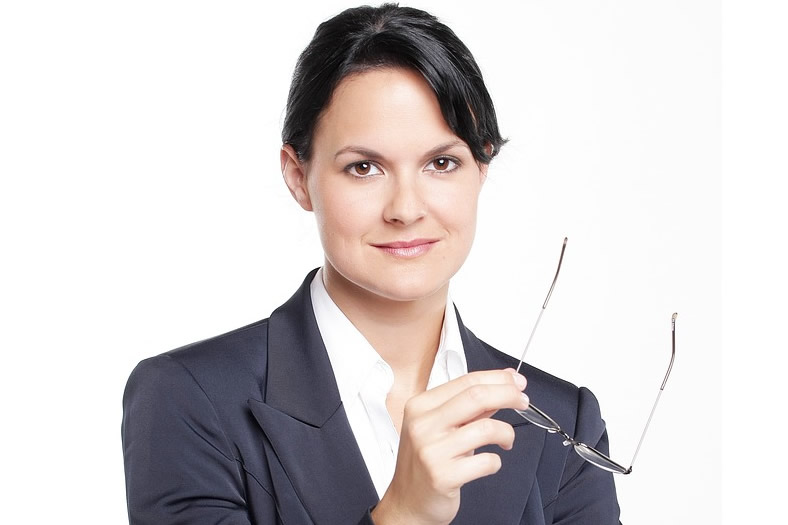
\includegraphics[width=0.7\textwidth,height=\textheight]{img/severina.jpg}
\caption{Severina Millanta}
\end{figure}

\begin{longtable}[]{@{}ll@{}}
\toprule
& Severina Millanta\tabularnewline
\midrule
\endhead
Età & 42\tabularnewline
Sesso & F\tabularnewline
Impiego & Ragioniera\tabularnewline
Figli & Una figlia di 10 anni\tabularnewline
Hobby & Cucina, nuoto\tabularnewline
Uso di internet & 80\% casa, 5\% lavoro, 15\% altrove\tabularnewline
\bottomrule
\end{longtable}

\hypertarget{personaggi-secondari}{%
\subsection{Personaggi secondari}\label{personaggi-secondari}}

\hypertarget{antonio-frastani}{%
\subsubsection{Antonio Frastani}\label{antonio-frastani}}

\begin{longtable}[]{@{}ll@{}}
\toprule
& Antonio Frastani\tabularnewline
\midrule
\endhead
Sesso & M\tabularnewline
Impiego & Impiegato bancario\tabularnewline
Figli & No\tabularnewline
Hobby & Motori\tabularnewline
Uso di internet & 70\% casa 20\% ufficio 10\% altro\tabularnewline
\bottomrule
\end{longtable}

\begin{figure}[h]
\centering
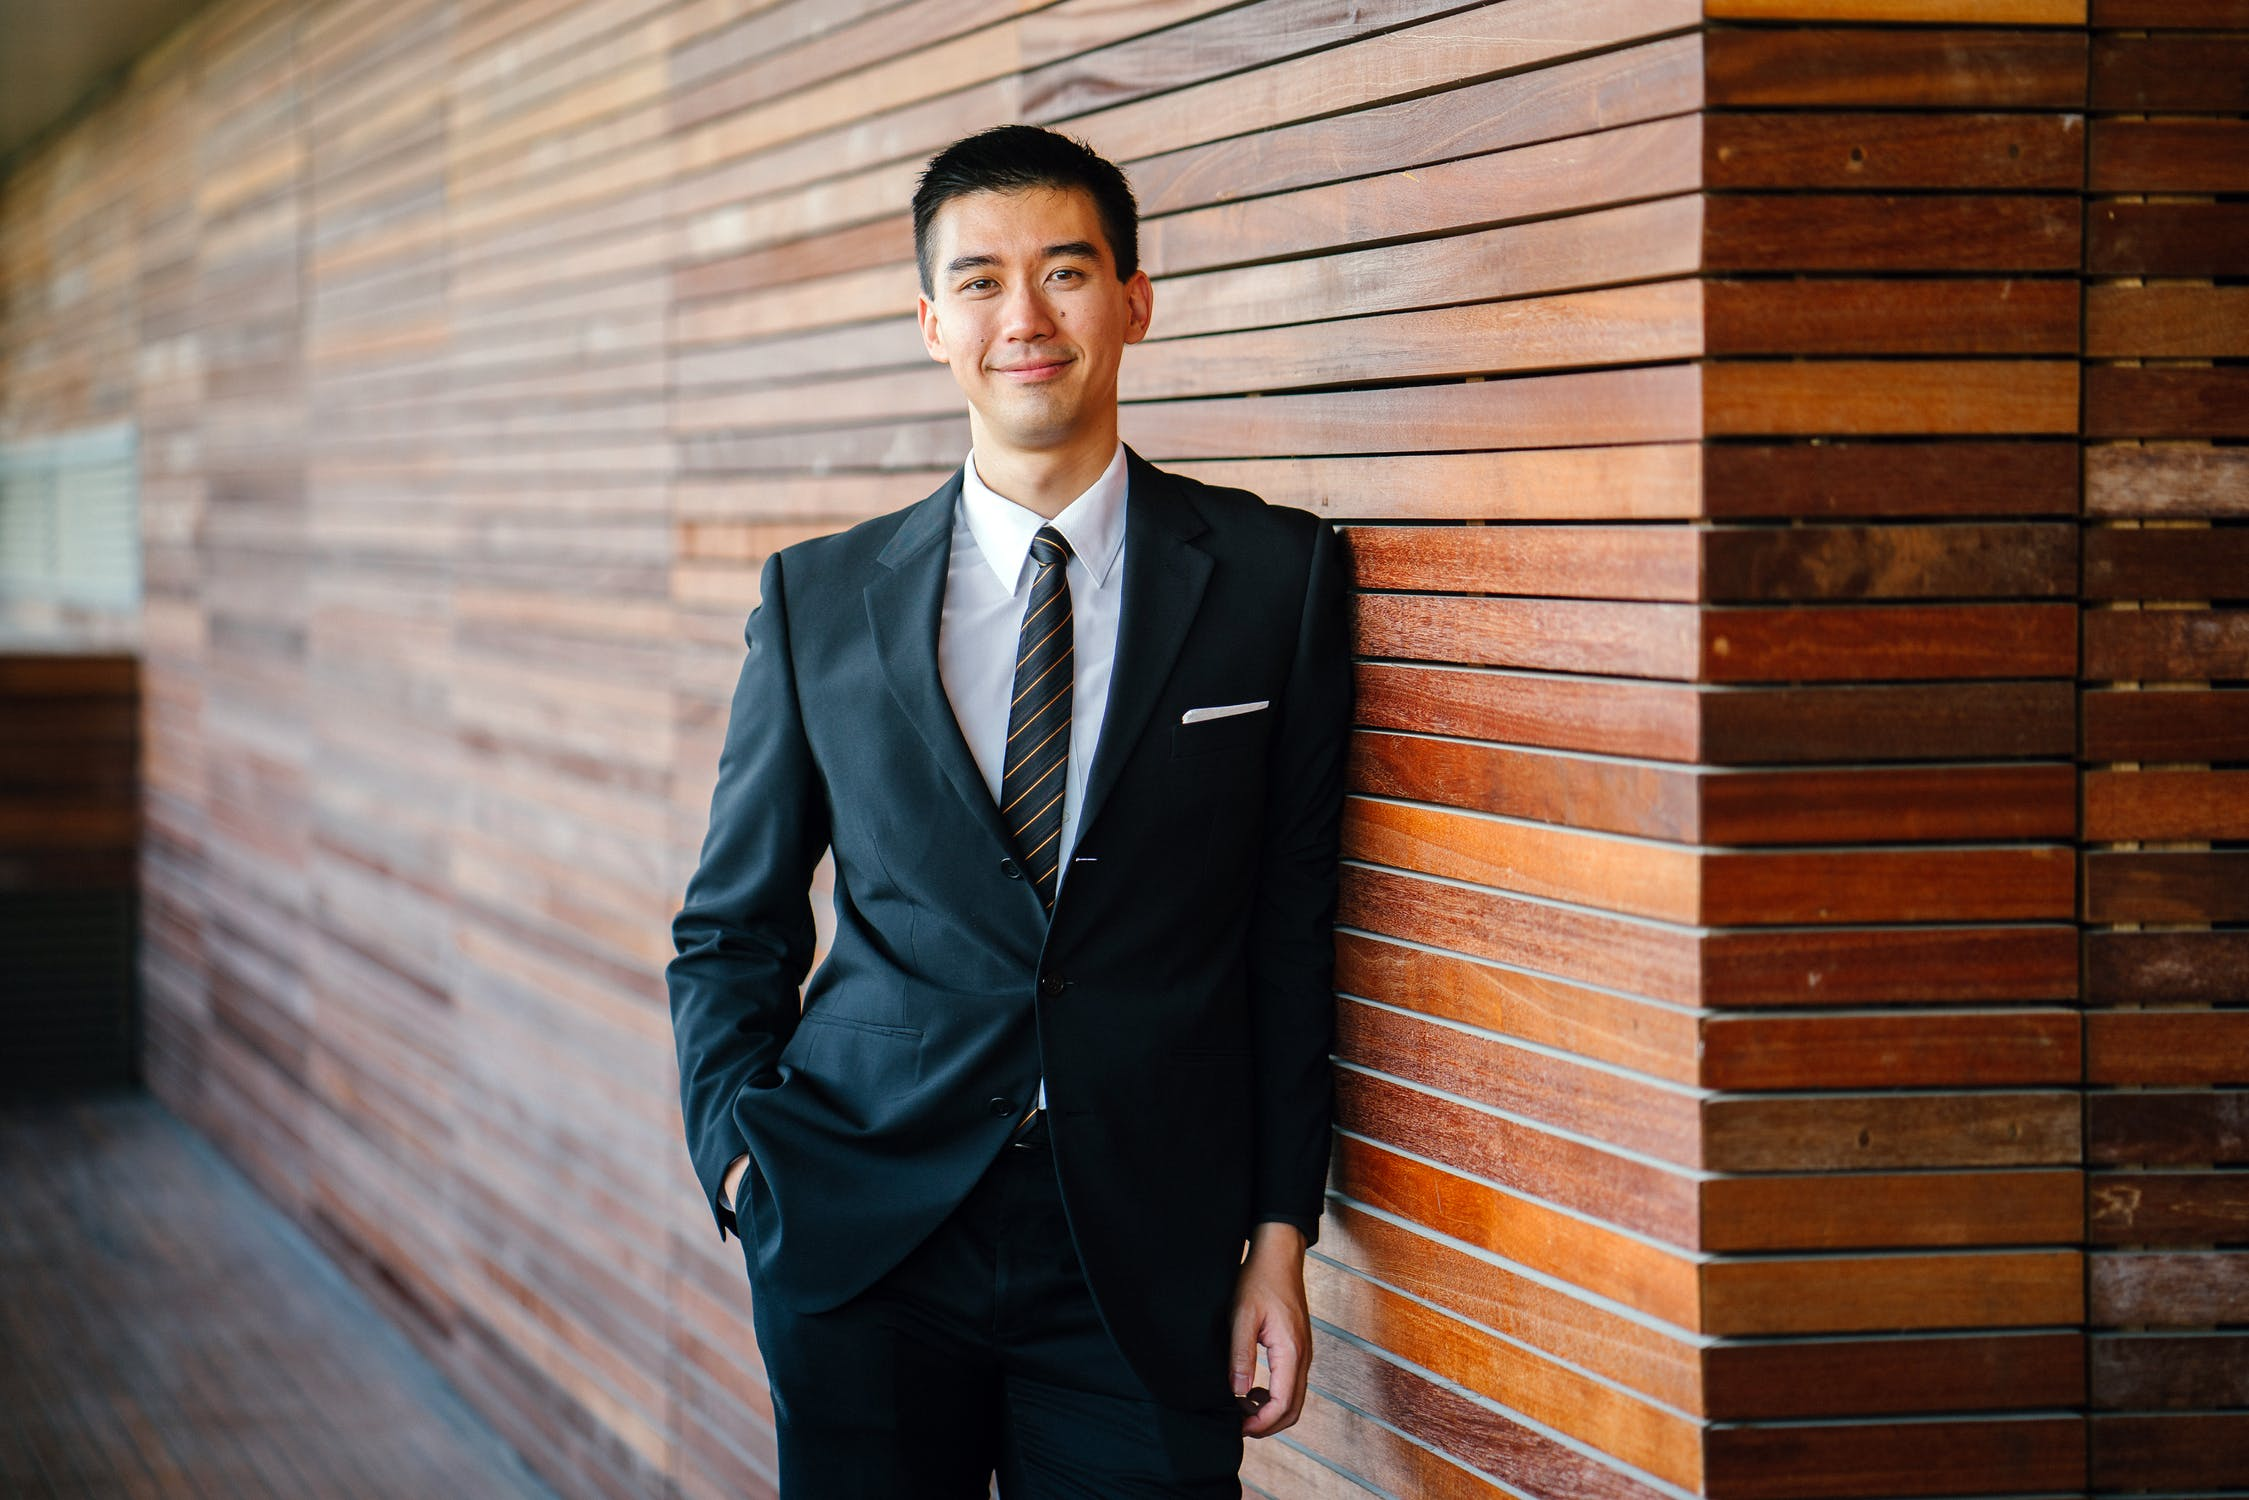
\includegraphics[width=0.7\textwidth,height=\textheight]{img/antonio.jpeg}
\caption{Antonio Frastani}
\end{figure}

\hypertarget{diego-de-la-vega}{%
\subsubsection{Diego de la Vega}\label{diego-de-la-vega}}

\begin{figure}[h]
\centering

\includegraphics[width=0.6\textwidth,height=\textheight]{img/diego.jpg}
\caption{Diego De La Vega}
\end{figure}

\begin{longtable}[]{@{}ll@{}}
\toprule
& Diego de la Vega\tabularnewline
\midrule
\endhead
Sesso & M\tabularnewline
Impiego & Personal Trainer\tabularnewline
Figli & No\tabularnewline
Hobby & Sport\tabularnewline
Uso di internet & 60\% lavoro 30\% casa 10\% altro\tabularnewline
\bottomrule
\end{longtable}

\hypertarget{elisa-pezzana}{%
\subsubsection{Elisa Pezzana}\label{elisa-pezzana}}

\begin{figure}[h]
\centering

\includegraphics[width=0.7\textwidth,height=\textheight]{img/elisa.jpg}
\caption{Elisa Pezzana}
\end{figure}

\begin{longtable}[]{@{}ll@{}}
\toprule
& Elisa Pezzana\tabularnewline
\midrule
\endhead
Sesso & F\tabularnewline
Impiego & Segretaria comunale\tabularnewline
Figli & Due: maschio, 14 anni e femmina, 12 anni\tabularnewline
Hobby & Palestra, shopping\tabularnewline
Uso di internet & 90\% lavoro 10\% altrove\tabularnewline
\bottomrule
\end{longtable}

\hypertarget{giorgia-moro}{%
\subsubsection{Giorgia Moro}\label{giorgia-moro}}

\begin{figure}[h]
\centering

\includegraphics[width=0.7\textwidth,height=\textheight]{img/giorgia.jpg}
\caption{Giorgia Moro}
\end{figure}

\begin{longtable}[]{@{}ll@{}}
\toprule
& Giorgia Moro\tabularnewline
\midrule
\endhead
Sesso & F\tabularnewline
Impiego & Impiegata contabile\tabularnewline
Figli & Una: femmina di 8 anni\tabularnewline
Hobby & Moda, antiquariato\tabularnewline
Uso di internet & 50\% lavoro 30\% casa 20\% altro\tabularnewline
\bottomrule
\end{longtable}

\hypertarget{proposta-di-progettazione}{%
\chapter{Proposta di progettazione}\label{proposta-di-progettazione}}

\hypertarget{architettura-dellinformazione}{%
\section{Architettura
dell'informazione}\label{architettura-dellinformazione}}

\hypertarget{modello-caos}{%
\section{Modello CAO=S}\label{modello-caos}}

Per cercare di soddisfare i bisogni dell'utente, data anche la poca
esperienza del gruppo e le limitazioni economiche, si è scelto di
utilizzare il modello di design \emph{goal-oriented CAO=S} che ci
consente di eliminare i task irrilevanti, poiché punta a raggiungere gli
obiettivi dell'utente, evitando gli errori più comuni nella
progettazione di sistemi usabili.

Le componenti principali del modello sono: ​Concetti, Attori​,
Operazioni​ e Strutture​. Tale modello studia i tipi di informazione
(Concetti) e mette a disposizione dei comandi (Operazioni) che
l'applicazione manipola per conto degli utenti (Attori), creando così
Strutture che vengono gestite dal modello.

\hypertarget{concetti}{%
\subsection{Concetti}\label{concetti}}

I concetti rappresentano il tipo di informazione che viene trattato e
quindi il modo in cui gli utenti percepiscono l'organizzazione delle
informazioni gestite dall'applicazione.

Sono un parametro fondamentale poiché esprimono i concetti con cui gli
utenti andranno ad interagire e una buona organizzazione risulta molto
utile quando sono presenti molte informazioni per evitare ambiguità
lessicali, concettuali, problemi di normalizzazione o altro.

È stato deciso quindi di usare i seguenti come concetti per evitare
fraintendimenti (essendo costituiti da un nome autoesplicativo, tali
concetti sono quindi sufficienti avere una comprensione base del
dominio): ERR

\begin{enumerate}
\def\labelenumi{\arabic{enumi}.}
\tightlist
\item
  \textbf{Creazione modello}
\item
  \textbf{Catalogo}
\item
  \textbf{Più votati}
\item
  \textbf{Progetto personale}
\item
  \textbf{Aiuto} ??? Andrebbe aggiunto un punto dove l'utente può
  chiedere aiuto? ERR
\end{enumerate}

\hypertarget{attori}{%
\subsection{Attori}\label{attori}}

Gli attori sono le categorie di utenti che agiscono sulle interfacce
dell'applicazione per svolgere i loro task manipolando le strutture dati
che loro interpretano come concetti. Non vengono rappresentati tramite
le proprie caratteristiche personali, ma per il ruolo che svolgono
all'interno dell'applicazione, che differenzia quindi l'interazione che
il sistema deve proporre.

In questa fase vengono definiti gli attori che interagiscono con il
sistema e si suddividono in \textbf{diretti}​, ovvero coloro che
useranno personalmente il sistema, ed \textbf{indiretti​}, ovvero coloro
che possono definire delle caratteristiche del sistema senza usare
direttamente l'interfaccia.

Dopo aver individuato gli attori diretti, ne vengono delineati i profili
rappresentandoli tramite un​ diagramma di strategia​, in cui vengono
analizzate caratteristiche e competenze attraverso un valore in una
scala che varia da 1 (valore molto basso) a 5 (valore molto alto),
quali:

\begin{itemize}
\tightlist
\item
  \textbf{Competenze tecniche}
\item
  \textbf{Competenze di dominio}
\item
  \textbf{Competenze linguistiche}
\item
  \textbf{Capacità fisiche}
\item
  \textbf{Motivazione}
\item
  \textbf{Concentrazione}
\end{itemize}

\hypertarget{severina-millanta-1}{%
\subsubsection{Severina Millanta}\label{severina-millanta-1}}

\begin{figure}[h]
\centering
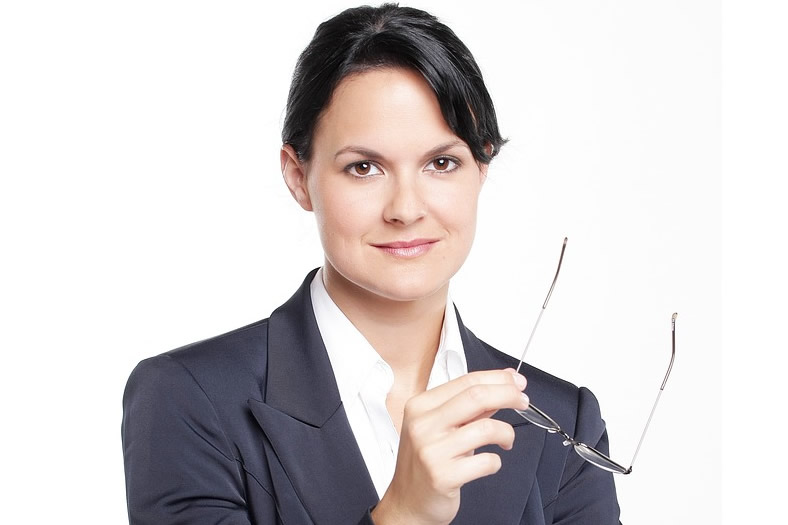
\includegraphics[width=0.5\textwidth,height=\textheight]{img/severina.jpg}
\caption{Severina Millanta}
\end{figure}

Severina ha preso il diploma da ragioniera ed è da allora che lavora
nello studio di un commercialista. Ha conosciuto suo marito poco tempo
in una cena aziendale. Hanno avuto una bambina e sono andati a vivere
insieme. Essendo entrambi lavoratori sono stati costretti ad avere una
babysitter per diversi anni. Ora la bambina ha 10 anni e Severina cerca
di passare più tempo possibile con lei.

Anche se la bambina cresce in fretta, lei adora fare shopping per la
piccola: non bada a spese, ma quello che le interessa di più e
l'originalità dei capi. Riserva la ricerca della qualità maggiore per
gli abitini domenicali, insomma le cose che non usa tutti i giorni.
Solitamente compra le taglie per la stagione attuale perché non vuole
vedere la roba tutta ammucchiata nei box o scaffali.

\begin{figure}[h]
\centering
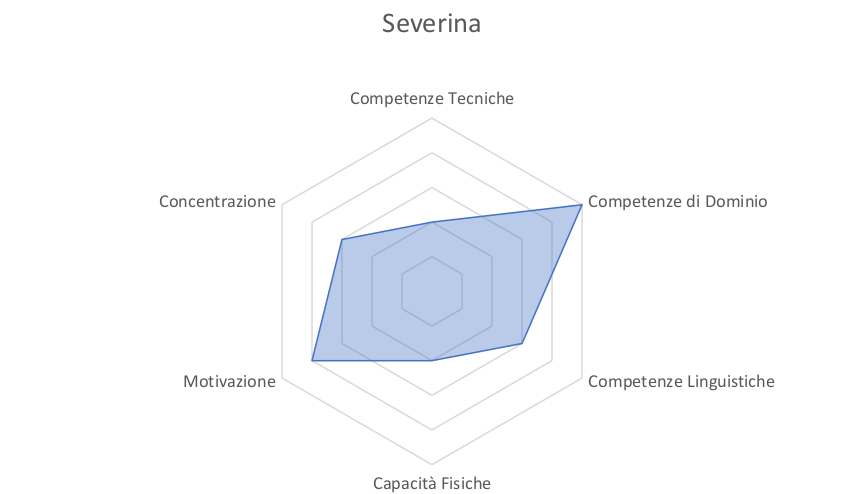
\includegraphics[width=0.5\textwidth,height=\textheight]{img/severina_competenze.png}
\caption{Severina Competenze}
\end{figure}

\hypertarget{antonio-frastani-1}{%
\subsubsection{Antonio Frastani}\label{antonio-frastani-1}}

\begin{figure}[h]
\centering
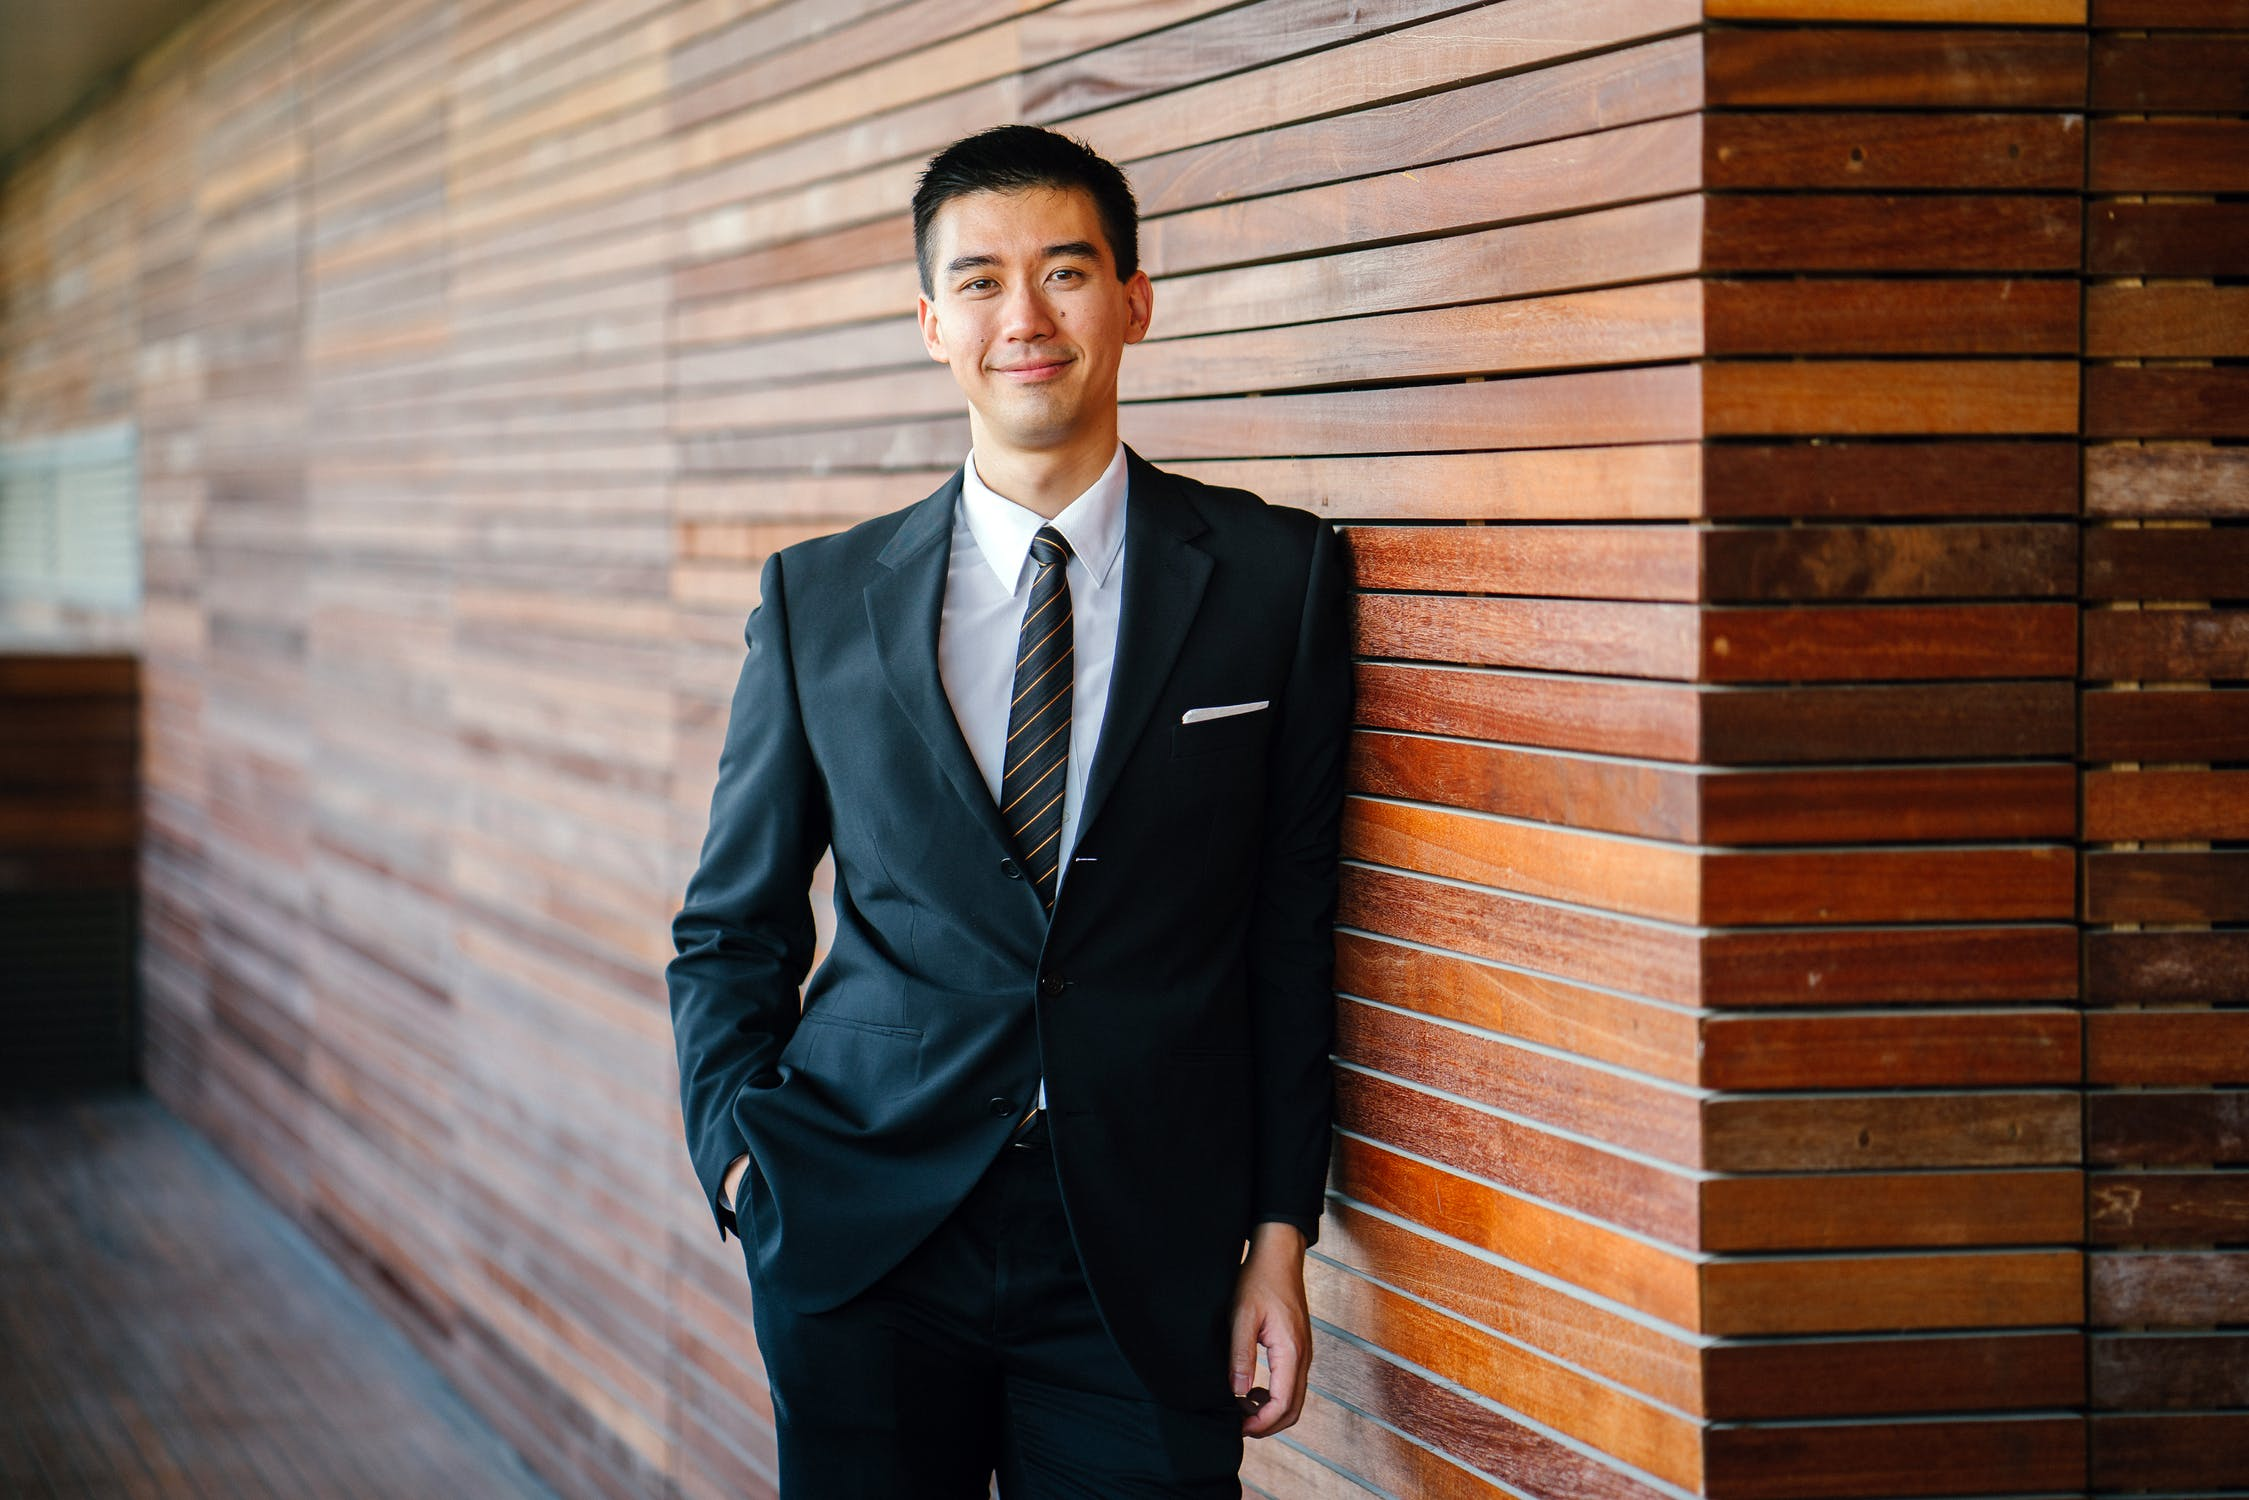
\includegraphics[width=0.5\textwidth,height=\textheight]{img/antonio.jpeg}
\caption{Antonio Frastani}
\end{figure}

Antonio è un giovane uomo di Firenze. Ha 27 anni e lavora da un anno
circa in una banca locale. Ama il suo lavoro, forse anche grazie allo
stipendio compreso tra i 25K e i 30K. Le sue competenze informatiche
sono ridotte: in ufficio utilizza il PC solo con programmi settoriali e
per redigere documenti, mentre a casa sfrutta il suo iPad Pro 2 per
navigare in rete e visitare i suoi amatissimi social networks. Antonio
adora le macchine e passa quasi tutto il suo tempo libero a vedere
programmi specializzati sull'argomento, raccogliere notizie in rete e
gestisce una pagina Facebook chiamata ``Motori in fiamme''.

\begin{figure}[h]
\centering
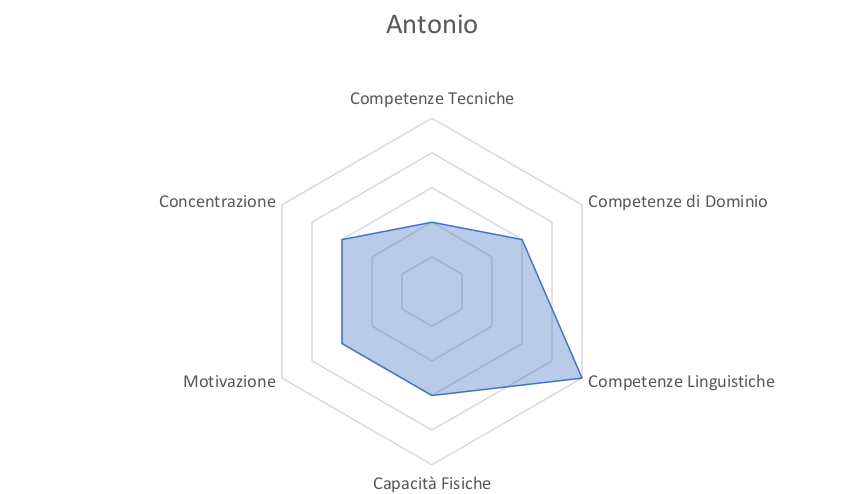
\includegraphics[width=0.5\textwidth,height=\textheight]{img/antonio_competenze.png}
\caption{Antonio Competenze}
\end{figure}

\hypertarget{diego-de-la-vega-1}{%
\subsubsection{Diego de la Vega}\label{diego-de-la-vega-1}}

\begin{figure}[h]
\centering

\includegraphics[width=0.6\textwidth,height=\textheight]{img/diego.jpg}
\caption{Diego de la Vega}
\end{figure}

Diego ha 26 anni, vive in un appartamento a Trento insieme alla mamma
Adriana di 56 anni, alla sorella Sofia di 28 e al nipotino Pietro di 5
anni. Ha una laurea triennale in Scienze Motorie conseguita
all'università telematica Pegaso.

Lavora da 2 anni nella palestra Body Planet di Trento come personal
trainer. In particolare si occupa di gestire i programmi fitness
individuali dei clienti, motivandoli e guidandoli nel raggiungimento dei
propri obiettivi. Sul posto di lavoro è molto preciso e professionale.
Va d'accordo con tutti i suoi colleghi PT con i quali è solito
scambiarsi consigli e opinioni. Al momento la palestra gli sta pagando
un corso di ginnastica posturale per migliorare la sua preparazione e
renderla più completa. Il suo sport preferito è il basket e non perde
occasione per andare allo stadio a fare il tifo per gli Aquila Basket
Trento.

I suoi obiettivi sono di riuscire ad aprire una palestra in cui
insegnare e applicare le tecniche dell'allenamento funzionale e di
trasferirsi a vivere da solo in un appartamento nella periferia
torinese, lontano dal traffico e dalla confusione della metropoli.

Diego utilizza il computer ogni giorno, sia al lavoro, per tenere
monitorata tutta l'attività riguardante i clienti, dalle schede di
allenamento, alla fatturazione, tramite l'applicativo PT Software 2.0,
sia a casa, per studiare, giocare, fare ricerche e molto altro. Per
quanto riguarda lo smartphone, l'unico uso che ne fa è per gestire i
suoi profili social. Percepisce uno stipendio lordo annuo di 25000 €.

\begin{figure}[h]
\centering
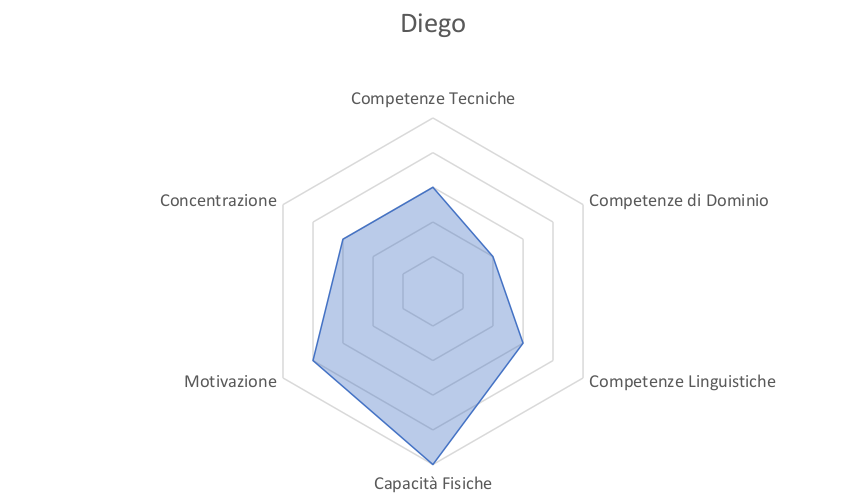
\includegraphics[width=0.5\textwidth,height=\textheight]{img/diego_competenze.png}
\caption{Diego Competenze}
\end{figure}

\hypertarget{elisa-pezzana-1}{%
\subsubsection{Elisa Pezzana}\label{elisa-pezzana-1}}

\begin{figure}[h]
\centering

\includegraphics[width=0.5\textwidth,height=\textheight]{img/elisa.jpg}
\caption{Elisa Pezzana}
\end{figure}

Elisa ha studiato economia a Bologna e dopo un paio di anni dalla laurea
ha vinto il concorso di segretaria comunale nel comune di residenza, è
sposata da 15 anni con Giorgio e hanno due figli. Elisa è una donna
solare, socievole e simpatica. Dimostra qualche anno in meno rispetto
alla sua età e le piace nuotare e cucinare Obiettivi: Organizzare le
vacanze estive con la famiglia.

Elisa il lunedi e il mercoledi va in palestra, il giovedi fa pilates con
le amiche e il martedi e venerdi va in piscina. La domenica mattina ha
l'abitudine di andare a fare colazione con le amiche al bar in centro
città.

\begin{figure}[h]
\centering
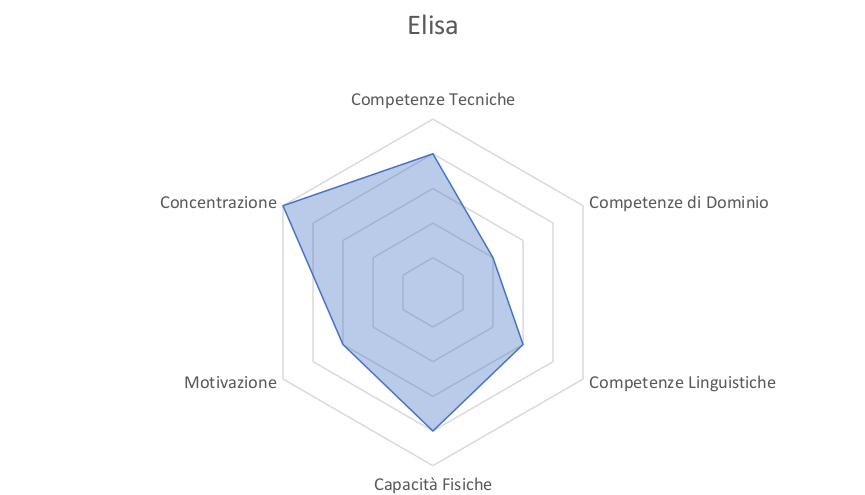
\includegraphics[width=0.5\textwidth,height=\textheight]{img/elisa_competenze.png}
\caption{Elisa Competenze}
\end{figure}

\hypertarget{giorgia-moro-1}{%
\subsubsection{Giorgia Moro}\label{giorgia-moro-1}}

\begin{figure}[h]
\centering

\includegraphics[width=0.5\textwidth,height=\textheight]{img/giorgia.jpg}
\caption{Giorgia Moro}
\end{figure}

Giorgia ha 38 anni, vive in un modesto appartamento a pochi chilometri
dal centro di Torino insieme alla sua famiglia. Ha una laurea triennale
in Economia e Commercio conseguita presso l'Università di Bologna. È
sposata con Andrea e hanno una figlia, Alice, di 8 anni.

Lavora da undici anni all'interno di un rinomato studio legale, operante
sia in Italia che all'estero, come impiegata contabile dove percepisce
uno stipendio lordo annuo di 36000€. Svolge il suo lavoro a stretto
contatto con gli altri membri dello studio, con i quali si confronta e
si scambiano idee, consigli e suggerimenti.

Utilizza raramente il PC, quasi esclusivamente per leggere email di
lavoro e guardare ricette da preparare per la famiglia. Ha una
certificazione di inglese di livello C1 conseguita al British Institutes
di Bologna, durante gli anni universitari, che le garantisce sia
un'ottima comprensione della lingua scritta e parlata sia un'ottima
capacità di scrittura. Da circa 3 mesi lo studio le sta pagando un corso
online sul GDPR.

Quando non lavora, a Giorgia piace navigare in rete con il suo
smartphone e tenere sempre aggiornato il suo profilo Facebook e
Instagram. Da diversi anni ha un abbonamento online a Vanity Fair,
attraverso il quale si tiene aggiornata sulle ultime tendenze. Nel tempo
libero le piace andare a visitare i mercatini d'antiquariato nella
periferia torinese, insieme alla figlia Alice, per cercare oggetti unici
e originali.

L'obiettivo di Giorgia è di comprare un nuovo appartamento, più grande e
più vicino al centro di Torino, e arredarlo con mobili e oggetti
d'antiquariato.

\begin{figure}[h]
\centering
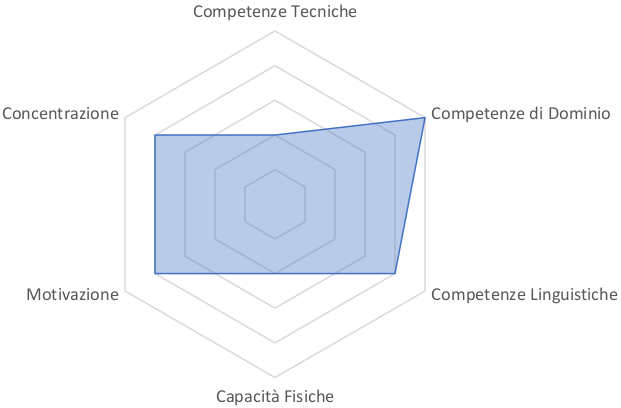
\includegraphics[width=0.5\textwidth,height=\textheight]{img/giorgia_competenze.png}
\caption{Giorgia Competenze}
\end{figure}

\hypertarget{operazioni}{%
\subsection{Operazioni}\label{operazioni}}

Nel modello CAO=S, le operazioni riguardano la manipolazione dei
concetti, elencati nella sezione precedente. La tipologia di operazioni
considerate sono quelle comunemente definite \emph{CRUD}: \emph{Create},
\emph{Read}, \emph{Update} e \emph{Delete}. Questo significa analizzare
le modalità di creazione, lettura, aggiornamento e rimozione dei
concetti elencati.

Ogni operazione è caratterizzata da determinate proprietà:

\hypertarget{creazione-nota-va-fatto-per-utente-loggato-e-non-loggato-err}{%
\subsubsection{Creazione {[}NOTA : va fatto per utente loggato e non
loggato{]}
ERR}\label{creazione-nota-va-fatto-per-utente-loggato-e-non-loggato-err}}

\begin{itemize}
\tightlist
\item
  \textbf{Tipo}: la creazione può esserre manuale, se avviene tramite un
  interazione con l'utente, automatica se è il sistema stesso ad
  aggiungere un elemento o implicita se viene eseguita dagli
  amministratori
\item
  \textbf{Valori di default}: lo stato iniziale con il quale un concetto
  viene valorizzato nel momento in cui viene aggiunto
\item
  \textbf{Moltiplicità}: singola o multipla a seconda della quantità di
  istanze che il sistema permette di inserire in una sola volta
\item
  \textbf{Persistenza}: indica la capacità di persistere o meno un
  istanza all'interno del sistema una volta che è stata aggiunta
\item
  \textbf{Memoria dell'utente}: in aggiunta ai valori di default, indica
  la presenza o meno di suggerimenti dati in base a valori inseriti in
  precedenza
\item
  \textbf{Notifiche di fallimento}: in caso di fallimento
  dell'operazione di salvataggio indica se ´e presente o meno un
  messaggio di errore.
\end{itemize}

\hypertarget{lettura}{%
\subsubsection{Lettura}\label{lettura}}

\begin{itemize}
\tightlist
\item
  Vista individuale \textbf{completa}: il concetto è visualizzato
  singolarmente in ogni suo dettaglio.
\item
  Vista individuale \textbf{ridotta}: i concetti sono visualizzati
  singolarmente e solo una parte delle loro informazioni è visibile
\item
  Vista \textbf{multipla}: permette la visualizzazione di più concetti
  contemporaneamente. Può essere una lista, che permette di visualizzare
  poche informazioni per ogni concetto, una lookup, attraverso la quale
  è possibile selezionare uno o più concetti per un uso futuro o un
  riassunto, usato per mostrare una descrizione non dettagliata di ogni
  concetto esposto
\end{itemize}

\hypertarget{aggiornamento}{%
\subsubsection{Aggiornamento}\label{aggiornamento}}

\begin{itemize}
\tightlist
\item
  \textbf{Globale}: tutte le proprietà di una determina istanza sono
  modificabili
\item
  \textbf{Specifico}: solo alcune delle proprietà di una determinata
  istanza sono modificabili
\end{itemize}

\hypertarget{eliminazione}{%
\subsubsection{Eliminazione}\label{eliminazione}}

\begin{itemize}
\tightlist
\item
  \textbf{Eliminazione}: l'entità viene completamente eliminata e non è
  più presente all'interno del sistema
\item
  \textbf{Archiviazione}: l'entità non viene del tutto eliminata, può
  essere ripristinata o eliminata definitivamente.
\end{itemize}

Il progetto proposto è un sottosito di contenuti, quindi le operazioni
effettuabili dagli attori principali sono solo ed esclusivamente di
visualizzazione. Le operazioni di creazione, aggiornamento e di
eliminazione sono già previste nel sito principale dell'azienda e non è
scopo di questo progetto trattarne le modalità. {[}DA RIDISCUTERE{]}

\begin{longtable}[]{@{}lllll@{}}
\toprule
\begin{minipage}[b]{0.17\columnwidth}\raggedright
\strut
\end{minipage} & \begin{minipage}[b]{0.17\columnwidth}\raggedright
Creazione\strut
\end{minipage} & \begin{minipage}[b]{0.17\columnwidth}\raggedright
Vista\strut
\end{minipage} & \begin{minipage}[b]{0.17\columnwidth}\raggedright
Aggiornamento\strut
\end{minipage} & \begin{minipage}[b]{0.17\columnwidth}\raggedright
Eliminazione\strut
\end{minipage}\tabularnewline
\midrule
\endhead
\begin{minipage}[t]{0.17\columnwidth}\raggedright
Modello\strut
\end{minipage} & \begin{minipage}[t]{0.17\columnwidth}\raggedright
Possibilità di creazione di un progetto per una maglietta\strut
\end{minipage} & \begin{minipage}[t]{0.17\columnwidth}\raggedright
Visione della maglietta durante la personalizzazione\strut
\end{minipage} & \begin{minipage}[t]{0.17\columnwidth}\raggedright
Modifica di un progetto t-shirt\strut
\end{minipage} & \begin{minipage}[t]{0.17\columnwidth}\raggedright
Eliminazione di un progetto t-shirt precedentemente creato\strut
\end{minipage}\tabularnewline
\begin{minipage}[t]{0.17\columnwidth}\raggedright
Progetti personali\strut
\end{minipage} & \begin{minipage}[t]{0.17\columnwidth}\raggedright
NO\strut
\end{minipage} & \begin{minipage}[t]{0.17\columnwidth}\raggedright
Visione di una o più magliette già creata da me\strut
\end{minipage} & \begin{minipage}[t]{0.17\columnwidth}\raggedright
Aggiornamento dei miei progetti personali\strut
\end{minipage} & \begin{minipage}[t]{0.17\columnwidth}\raggedright
NO\strut
\end{minipage}\tabularnewline
\begin{minipage}[t]{0.17\columnwidth}\raggedright
Catalogo\strut
\end{minipage} & \begin{minipage}[t]{0.17\columnwidth}\raggedright
NO\strut
\end{minipage} & \begin{minipage}[t]{0.17\columnwidth}\raggedright
Visione di una o più magliette creata da qualsiasi utente\strut
\end{minipage} & \begin{minipage}[t]{0.17\columnwidth}\raggedright
Votazione di un progetto (+1)\strut
\end{minipage} & \begin{minipage}[t]{0.17\columnwidth}\raggedright
NO\strut
\end{minipage}\tabularnewline
\begin{minipage}[t]{0.17\columnwidth}\raggedright
Più votati\strut
\end{minipage} & \begin{minipage}[t]{0.17\columnwidth}\raggedright
NO\strut
\end{minipage} & \begin{minipage}[t]{0.17\columnwidth}\raggedright
Visione dei progetti più votati\strut
\end{minipage} & \begin{minipage}[t]{0.17\columnwidth}\raggedright
NO\strut
\end{minipage} & \begin{minipage}[t]{0.17\columnwidth}\raggedright
NO\strut
\end{minipage}\tabularnewline
\bottomrule
\end{longtable}

\hypertarget{strutture}{%
\subsection{Strutture}\label{strutture}}

Una volta identificati gli utenti, i concetti e le operazioni, il passo
successivo di CAO=S consiste nella definizione delle strutture. Questo
avviene tramite la compilazione di tabelle tridimensionali che mostrano
come gli attori interagiscono con i vari contenuti usando le operazioni
descritte.

La tabella ha per assi i concetti, gli attori e le operazioni, e
all'interno di ogni cella si inseriscono delle annotazioni di come un
attore deve poter eseguire l'operazione sul concetto.

Ci sono tre tipi di strutture che interessano lo sviluppo:

\begin{itemize}
\tightlist
\item
  \textbf{Viste}: maschere di visualizzazione delle proprietà dei
  concetti
\item
  \textbf{Navigazione}: meccanismi di passaggio da una vista all'altra
\item
  \textbf{Strutture dati}: normalizzazione dello studio dei concetti in
  modelli di memorizzazione persistente delle entità
\end{itemize}

\begin{longtable}[]{@{}lllll@{}}
\toprule
Concetti & Creazione & Vista & Aggiornamento &
Eliminazione\tabularnewline
\midrule
\endhead
Modello & Editor & Visuale di dettaglio & Editor & Editor\tabularnewline
Catalogo & NO & Visione multipla & Votazione di un progetto (+1) &
NO\tabularnewline
Progetti personali & NO & Visione multipla & Editor & NO\tabularnewline
Più votati & NO & Visione multipla & NO & NO\tabularnewline
\bottomrule
\end{longtable}

\hypertarget{progettazione-dellinterazione}{%
\section{Progettazione
dell'interazione}\label{progettazione-dellinterazione}}

Lo scopo dell'applicazione è quello di fornire agli utenti uno store
online dove possano personalizzare una t-shirt ed avere la possibilità
di riceverla a casa.

L'interazione può essere vista come un dialogo tra utente e computer. La
scelta dello stile di interazione ha profondi effetti sulla natura del
dialogo e, di conseguenza, sull'efficacia dell'interazione.

Sono stati identificati sei principali stili di interazione:

\begin{itemize}
\tightlist
\item
  \textbf{Menu and navigation}
\item
  \textbf{Command entry}
\item
  \textbf{Question/Answer}
\item
  \textbf{Spreadsheet/form-fill}
\item
  \textbf{Natural language}
\item
  \textbf{Direct manipulation}
\end{itemize}

Ai fini del progetto é stato utilizzato principalmente lo stile ``Menu e
navigazione''. Esso permettere di organizzare i comandi i menu
gerarchici risolvendo il problema della visualizzazione di queste che,
quando numerose, possono arrivare ad occupare grossa parte dello
schermo.

Anche se questo tipo di interazione potrebbe rallentare gli utenti
esperti, in realtà, data la presenza di un numero di categorie e
sottocategorie limitate non impattare sulla velocità di esecuzione delle
operazioni.

Per quanto riguarda la disposizione fisica dei controlli si è deciso di
adottare un approccio con raggruppamenti funzionali, ossia, sono stati
raggruppati insieme i comandi che permettono interazioni correlate.

Per quanto riguarda la navbar in alto, sono presenti due sezioni.

La prima sezione appartiene al sito madre Kiabi e contiene:

\begin{itemize}
\tightlist
\item
  Logo: permette di identificare il sito ed ha un link che consente di
  tornare sempre alla pagina principale;
\item
  Barra di ricerca: permette di effettuare una query in linguaggio
  naturale per cercare tra gli articoli presenti nel catalogo. Vengono
  utilizzate tecniche come la query expansion per ampliare l'output di
  ricerca con sinonimi delle parole ricercate. Il risultato sarà una
  lista di articoli che soddisfano le richieste della query;
\item
  Profilo: permette l'accesso rapido alle informazioni dell'account,
  alle modalità di pagamento, agli ordini effettuati (appartiene al sito
  madre);
\item
  Whishlist: permette di salvare gli articoli di interesse senza
  caricarli nel carrello;
\item
  Carrello: permette di accedere alla lista di articoli pronti per
  essere acquistati;
\end{itemize}

La seconda sezione contiene il menu di navigazione e varia in funzione
della tipologia di utente. Per l'utente non loggato offre:

\begin{itemize}
\tightlist
\item
  Home: permette di accedere alla pagina principale del sottosito
\item
  Catalogo: permette di accedere al catalogo con la lista dei prodotti
  già personalizzati da tutti gli utenti
\item
  Più Votati: permette di accedere alla lista dei podotti più votati
\end{itemize}

Per l'utente loggato, oltre alle aree precedenti, si aggiungono:

\begin{itemize}
\tightlist
\item
  Progetti Personali: permette di accedere alla lista di prodotti
  personalizzati dall'utente stesso
\item
  Carica Modello: permette di caricare il modello di un prodotto
  precedentemente salvato sulla macchina dell'utente ERR
\end{itemize}

Esiste una ulteriore barra posta in basso che viene visualizzata solo
qualndo si è all'interno dell'editor. Essa ospita i link rapidi che
permettono di acquistare un prodotto (portando al carrello) o di
salvarlo nei progetti personali. Inoltre ospita un drop-up menu con la
lista delle modifiche selezionate.

{[}INSERIRE DESCRIZIONE MENU CHE APPARE QUANDO SI CLICCA SU
BAMBINO/BAMBINA{]} ERR

{[}INSERIRE DESCRIZIONE MENU DELL'EDITOR{]} ERR

Il footer (in basso) contiene informazioni sui contatti (telefonici ed
e-mail), varie informazioni su pagamenti, modalità di spedizione, aiuto,
FAQ e informazioni. Esso fa parte del sito madre kiabi.

\hypertarget{blueprints}{%
\section{Blueprints}\label{blueprints}}

Le blueprint sono semplici diagrammi che definiscono l'organizzazione
dei contenuti e come le varie componenti interagiscono tra di loro.

Saranno presentate quattro blueprint che mostrano rispettivamente:

\begin{enumerate}
\def\labelenumi{\arabic{enumi}.}
\tightlist
\item
  Organizzazione completa dei contenuti di Kids Experience
\item
  Creazione di un nuovo modello
\item
  Organizzazione delle azioni disponibili per un utente loggato
\item
  Organizzazione delle azioni disponibili per un utente non loggato
\end{enumerate}

\begin{figure}[h]
\centering
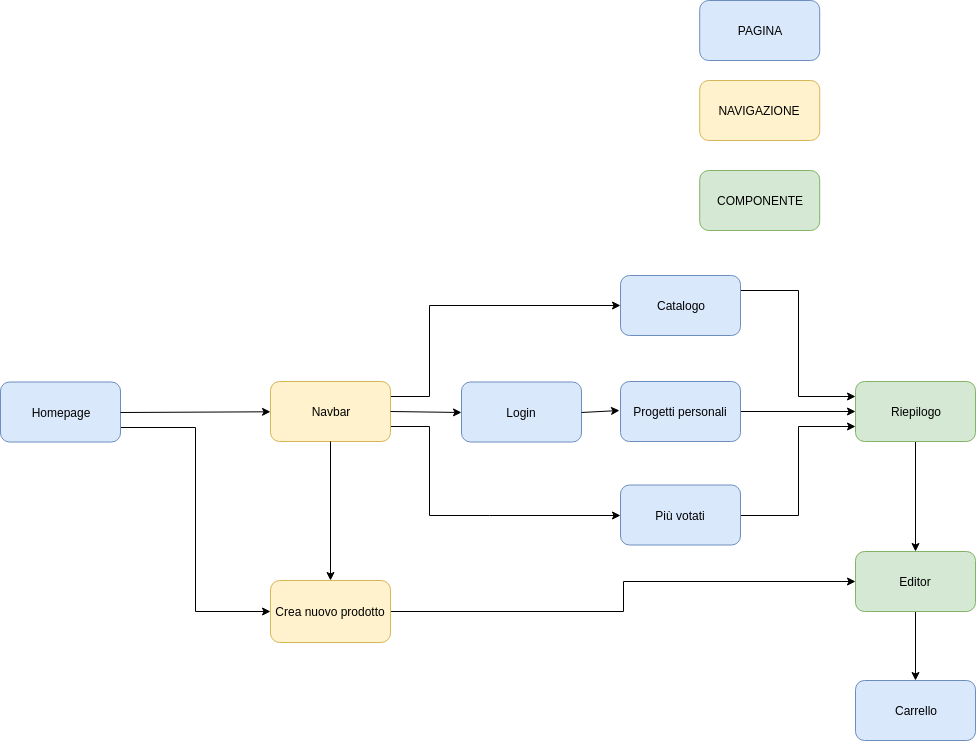
\includegraphics{img/Generale_Kids_Experience.png}
\caption{Generale}
\end{figure}

\begin{figure}[h]
\centering
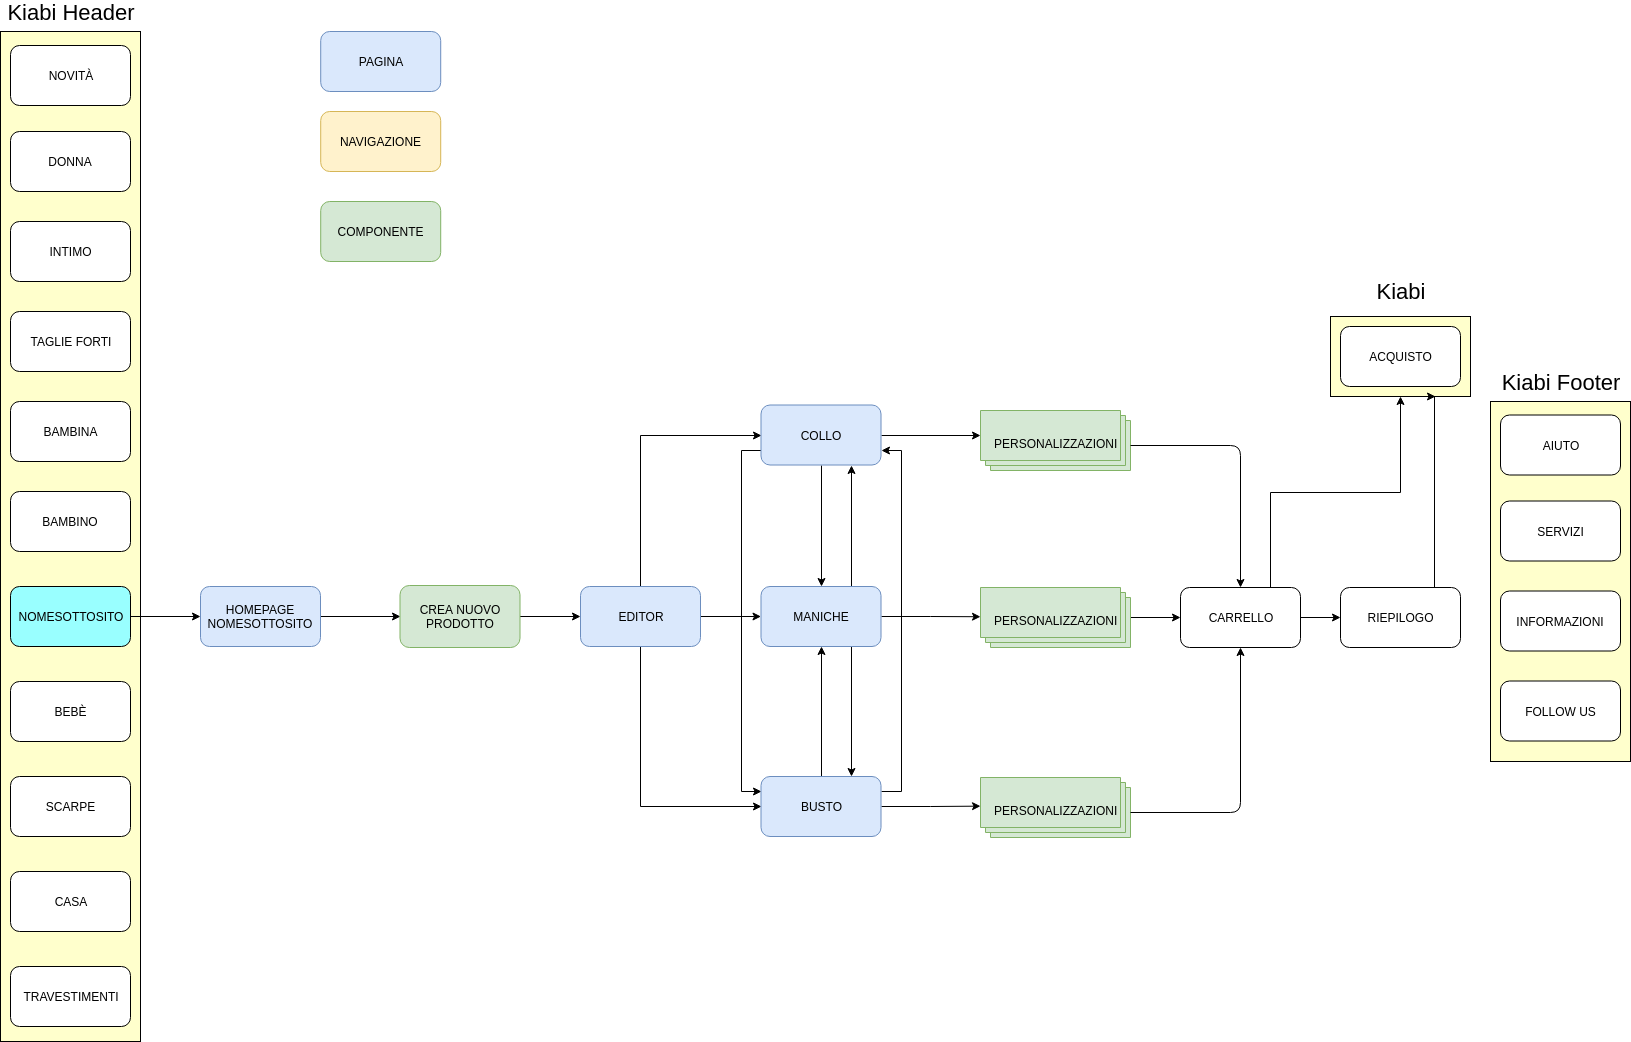
\includegraphics{img/Creazione_modello.png}
\caption{Creazione modello}
\end{figure}

\begin{figure}[h]
\centering
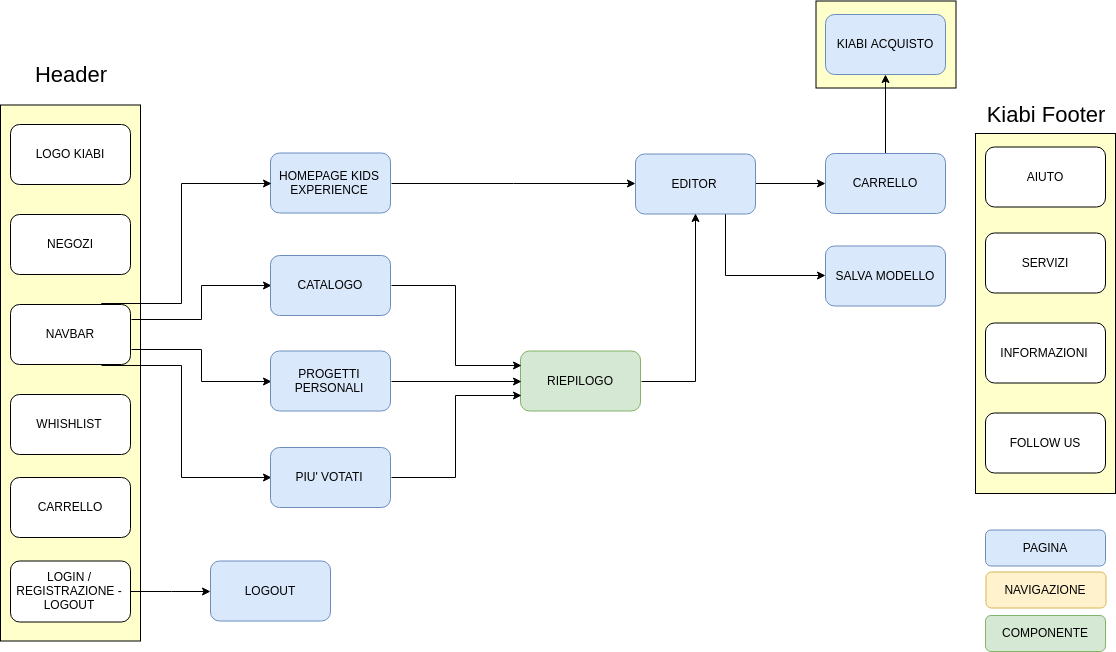
\includegraphics{img/Utente_loggato.png}
\caption{Utilizzo del sistema - Utente loggato}
\end{figure}

\begin{figure}[h]
\centering
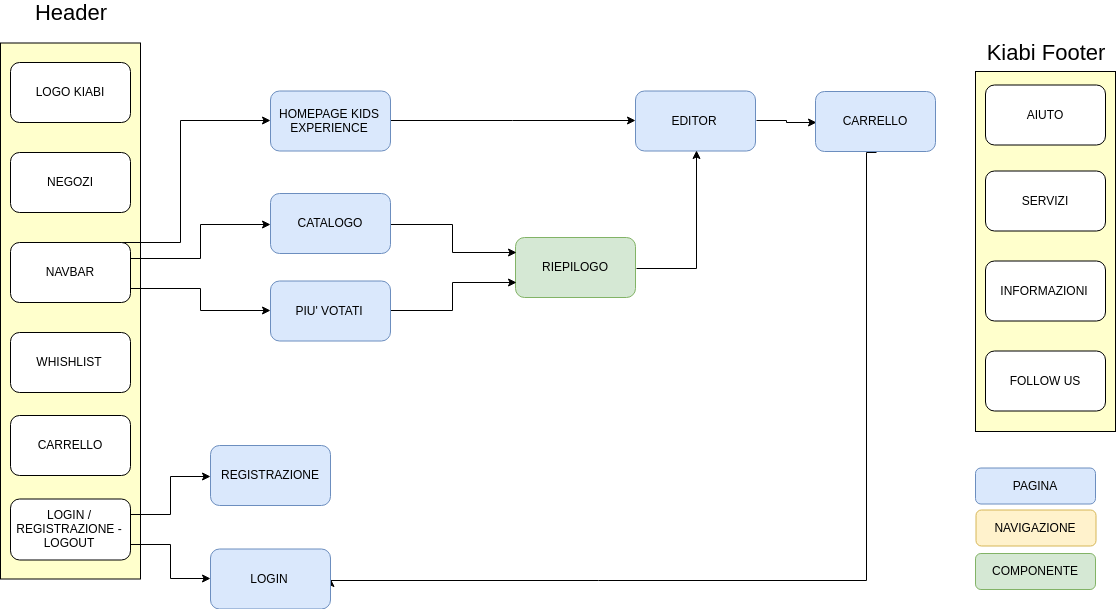
\includegraphics{img/Utente_non_loggato.png}
\caption{Utilizzo del sistema - Utente non loggato}
\end{figure}

\hypertarget{wireframes}{%
\section{Wireframes}\label{wireframes}}

I wireframe sono illustrazioni organizzative schematiche dei contenuti
presenti in un progetto. La funzione principale dei wireframe è di
comunicare l'idea del progetto, focalizzando l'attenzione
sull'architettura piuttosto che il design. Contengono i comandi
necessari per permettere all'utente di realizzare un task. Spesso sono
anche accompagnati da testo e immagini. Sono strumenti potenti che
permettono di effettuare test con gli utenti per la valutazione del
sistema e permettono di apportare modifiche restando ancora in fase di
prototipazione con conseguente risparmi di tempo e denaro.

\hypertarget{home}{%
\subsection{Home}\label{home}}

La Home di Kids Experience è divisa in tre sezioni: header, corpo e
footer. La pagina è scrollabile e l'header rimane sempre visibile in
quanto contiene elementi che garantiscono un accesso rapido alle altre
sezioni.

Il corpo ha una funzione prevalentemente informativa. Di fondamentale
importanza sono lo slogan e il bottone ``Crea!'' che permette un accesso
diretto all'editor.

Il footer, ereditato da Kiabi, contiente elementi marginali di
navigazione come: una sezione di aiuto, una di servizi, una sezione
informativa e i rimandi ai principali social network.

\begin{figure}[h]
\centering
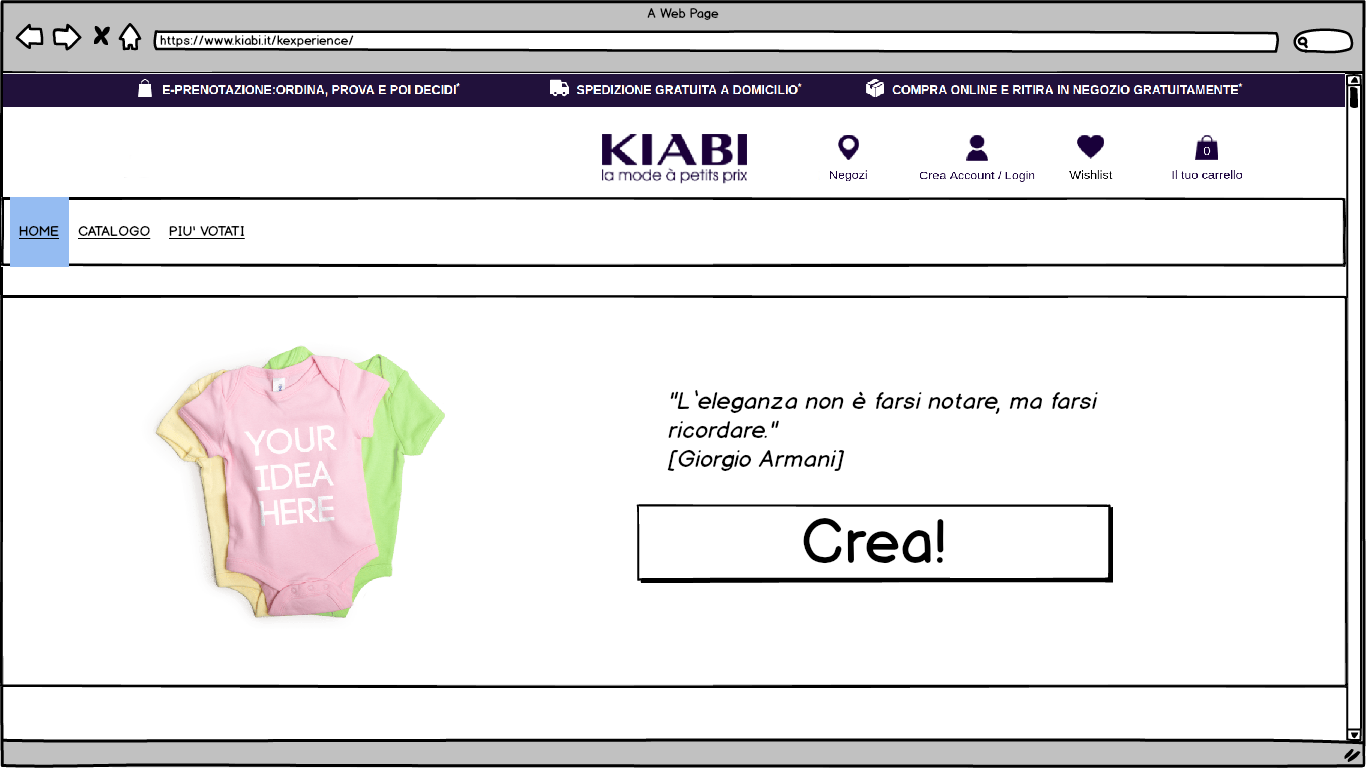
\includegraphics{img/balsamiq/HomeSottositoUtenteEsterno.png}
\caption{Utilizzo del sistema - Utente non loggato}
\end{figure}

\hypertarget{creazione-modello}{%
\subsection{Creazione modello}\label{creazione-modello}}

Il processo di creazione di una maglietta personalizzata si compone di
svariati passaggi data l'ampia gamma di personalizzazioni disponibili.
Sulla parte sinistra della schermata sono presenti le quattro
macrocategorie di personalizzazioni. Dall'altro lato è presentata
un'anteprima in tempo reale delle personalizzazioni applicate e una
miniatura che permette di invertire il lato visibile della maglietta,
permettendo una personalizzazione a 360°.

Tramite i link sulla sinistra è possibile accedere alle finestre di
dettaglio delle personalizzazioni. In ogni sezione dell'editor è
presente una navbar che permette un rapido accesso alle sezioni
principali di Kids Experience e di scaricare il progetto corrente in un
formato standard. Infine nell'header è presente una comoda barra di
ricerca che permette di cercare risultati sia nel catalogo di Kiabi che
in quello di Kids Experience.

\begin{figure}[h]
\centering
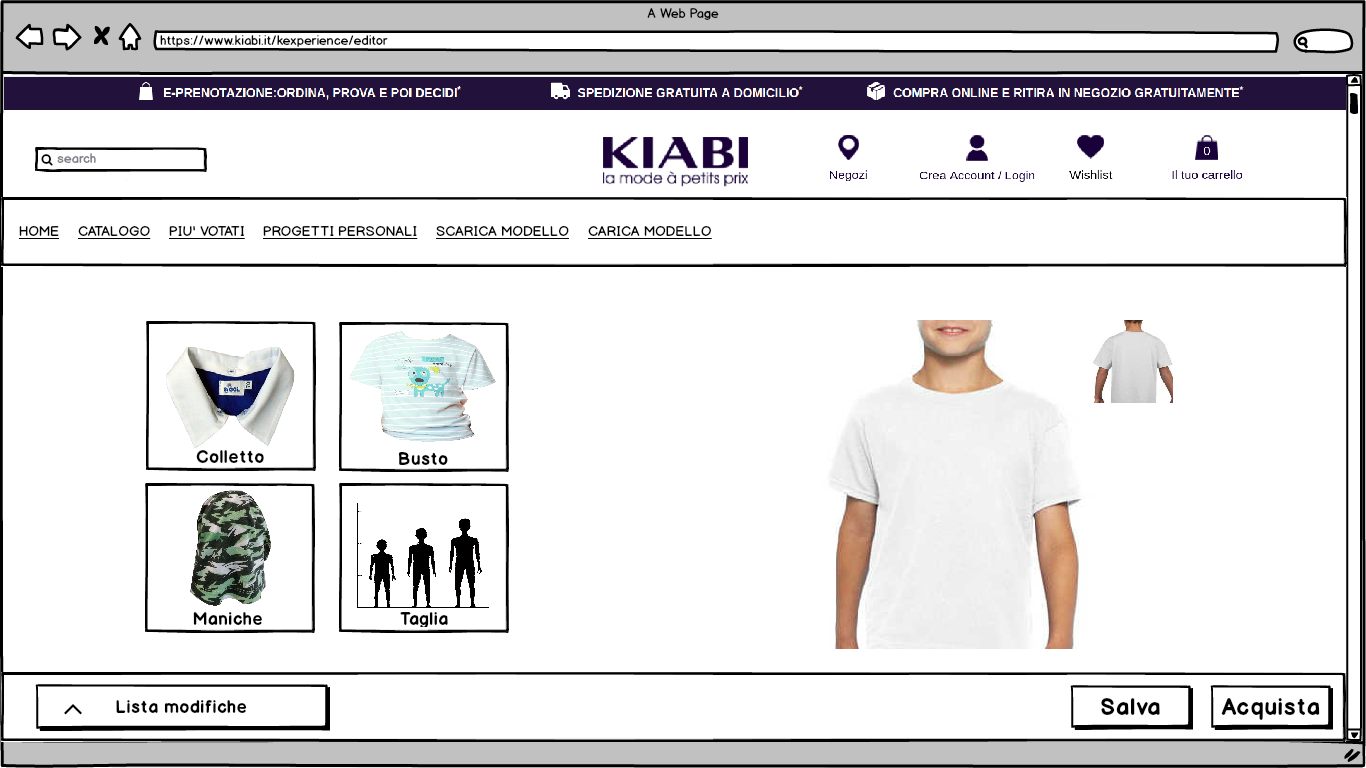
\includegraphics{img/balsamiq/Editorbase.png}
\caption{Editor}
\end{figure}

Ogni volta che viene inserita una personalizzazione, oltre ad essere
visualizzata direttamente sul modello, appare anche all'interno della
\textbf{lista delle modifiche}, insieme al costo unitario ed un'icona
per la rimozione. Il costo totale della maglietta e delle
personalizzazioni applicate è sempre ben visibile nella barra in basso.
Nella medesima barra sono presenti i bottoni per salvare il progetto
attuale nei progetti personali o per acquistarlo.

\begin{figure}[h]
\centering
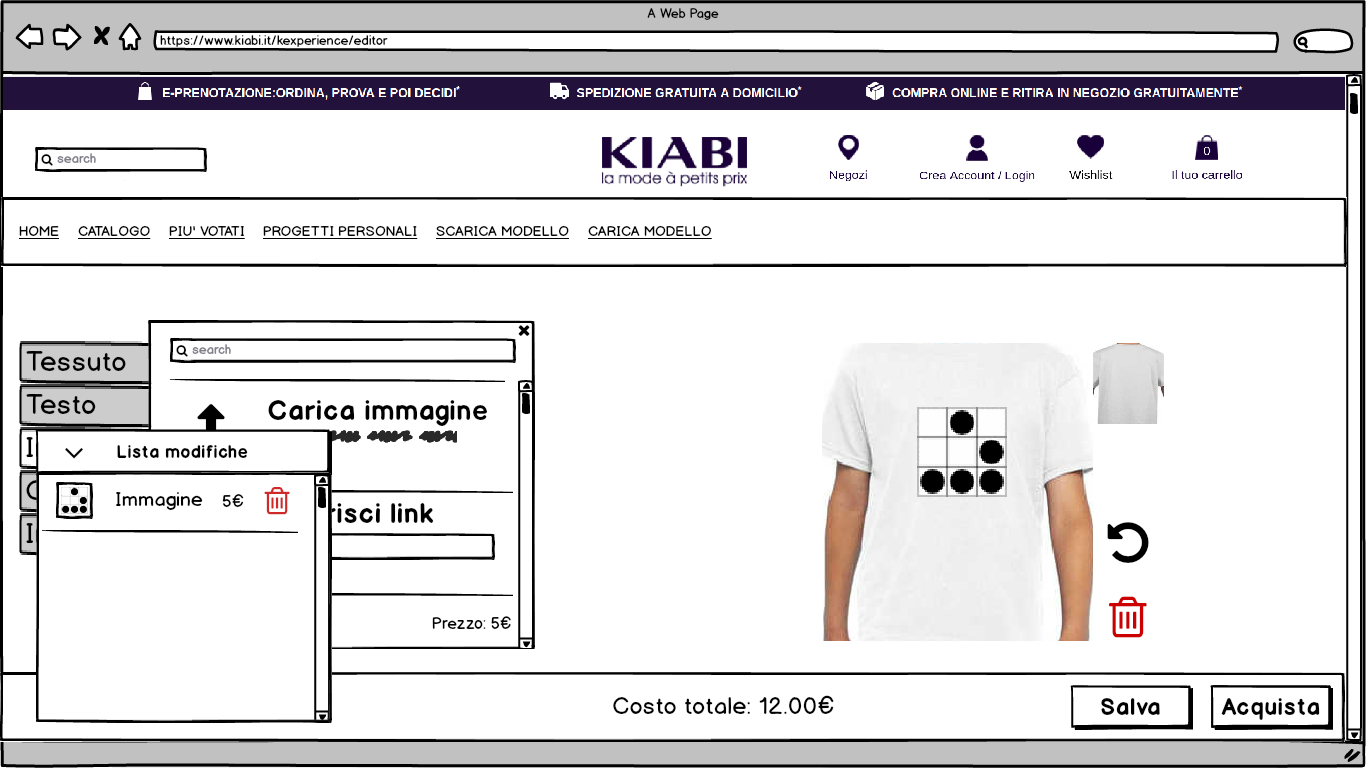
\includegraphics{img/balsamiq/Editor-caratteristicabustoimmagine4.png}
\caption{Editor - Inserimento immagine}
\end{figure}

Procendo con l'acquisto si giunge nella pagina del carrello. Qui
troviamo un riepilogo dei prodotti inseriti finora, con la possibilità
di modificarne il numero di pezzi.

\begin{figure}[h]
\centering
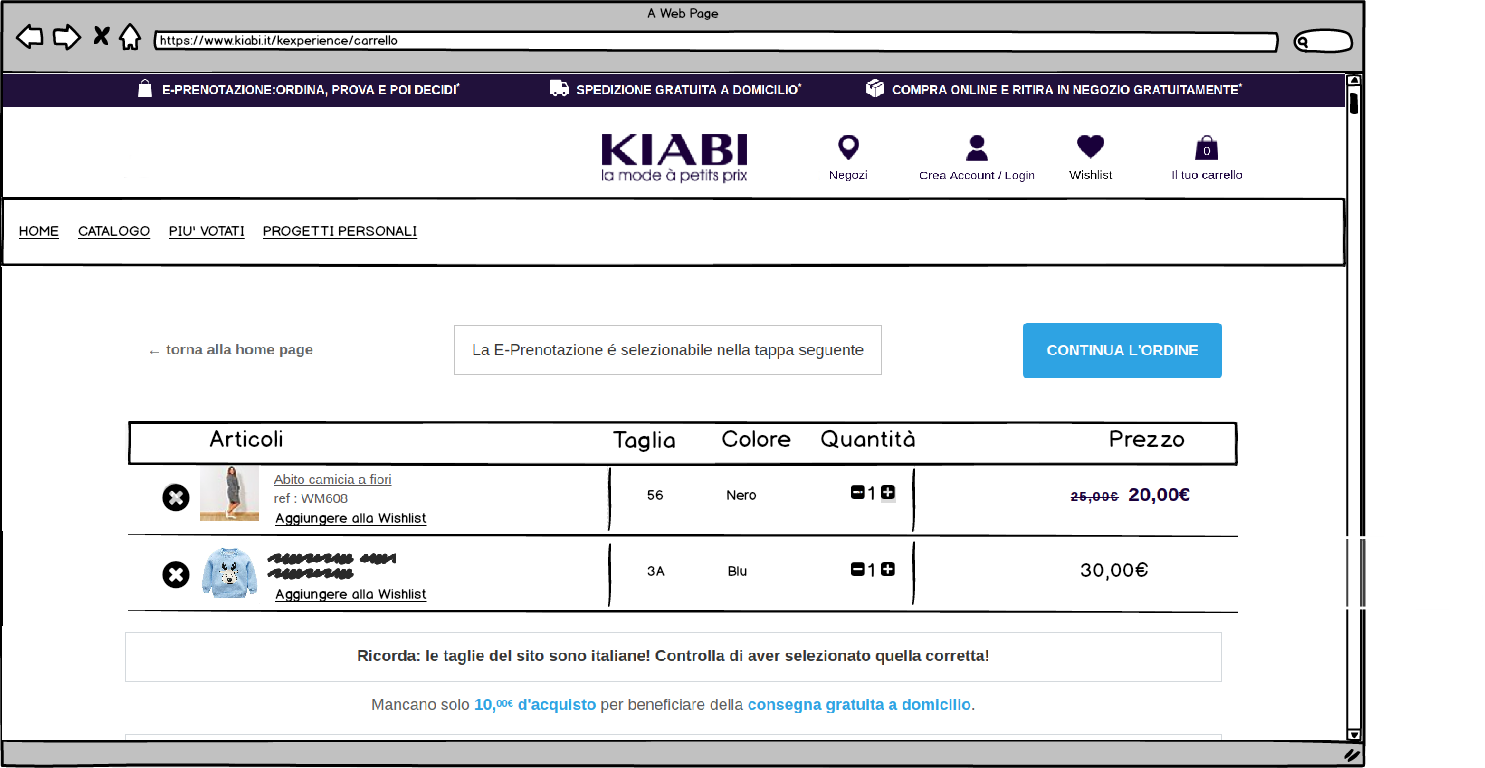
\includegraphics{img/balsamiq/Carrello.png}
\caption{Carrello}
\end{figure}

Premendo sulla miniatura di uno dei prodotti presenti nel carrello si
apre un modale in cui è presente una lista completa delle
personalizzazioni e relativi costi, il costo totale e un bottone che
permette di tornare all'editor per continuare la personalizzazione.

\begin{figure}[h]
\centering
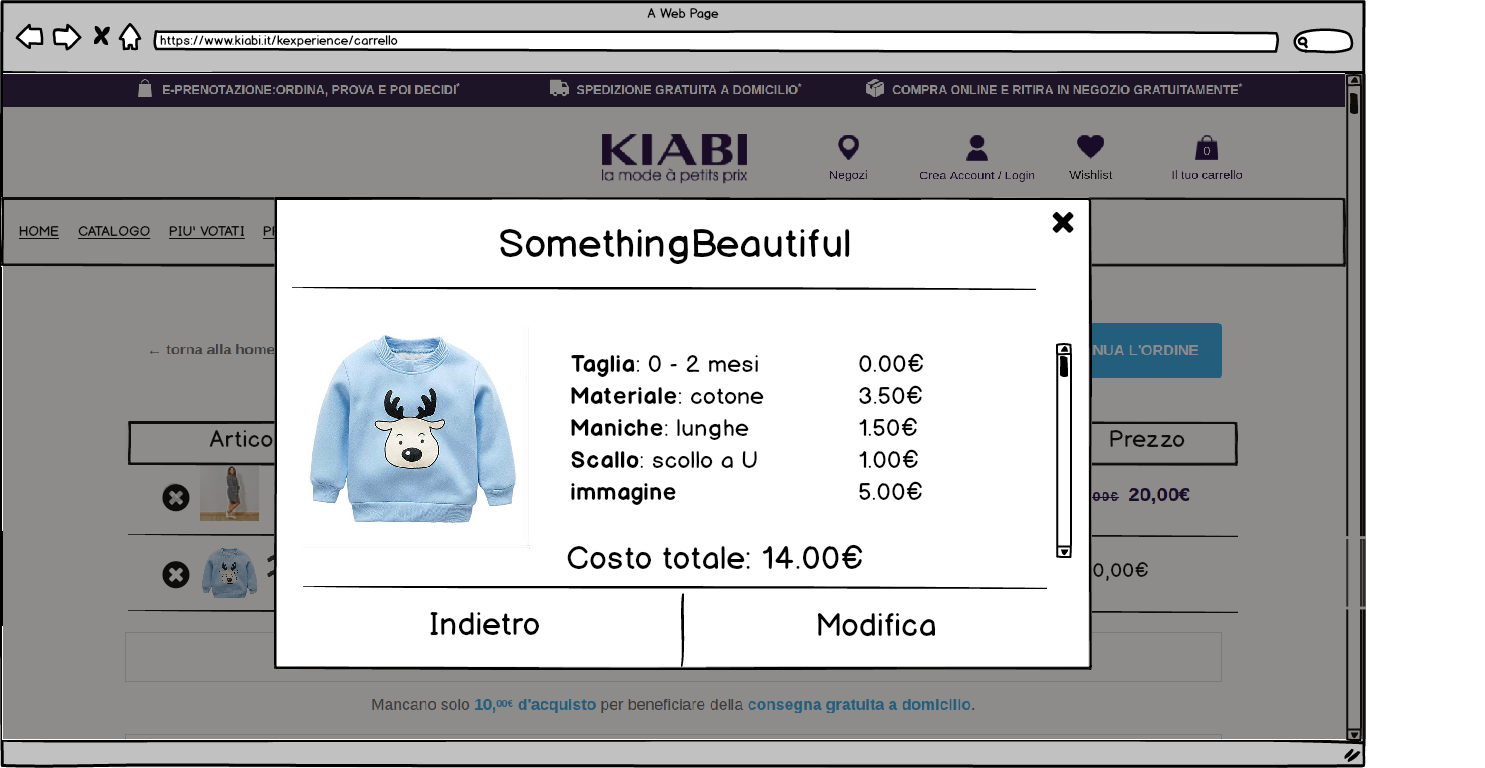
\includegraphics{img/balsamiq/Carrellodettagli.png}
\caption{Carrello - dettaglio}
\end{figure}

\hypertarget{catalogo}{%
\subsection{Catalogo}\label{catalogo}}

\begin{figure}[h]
\centering
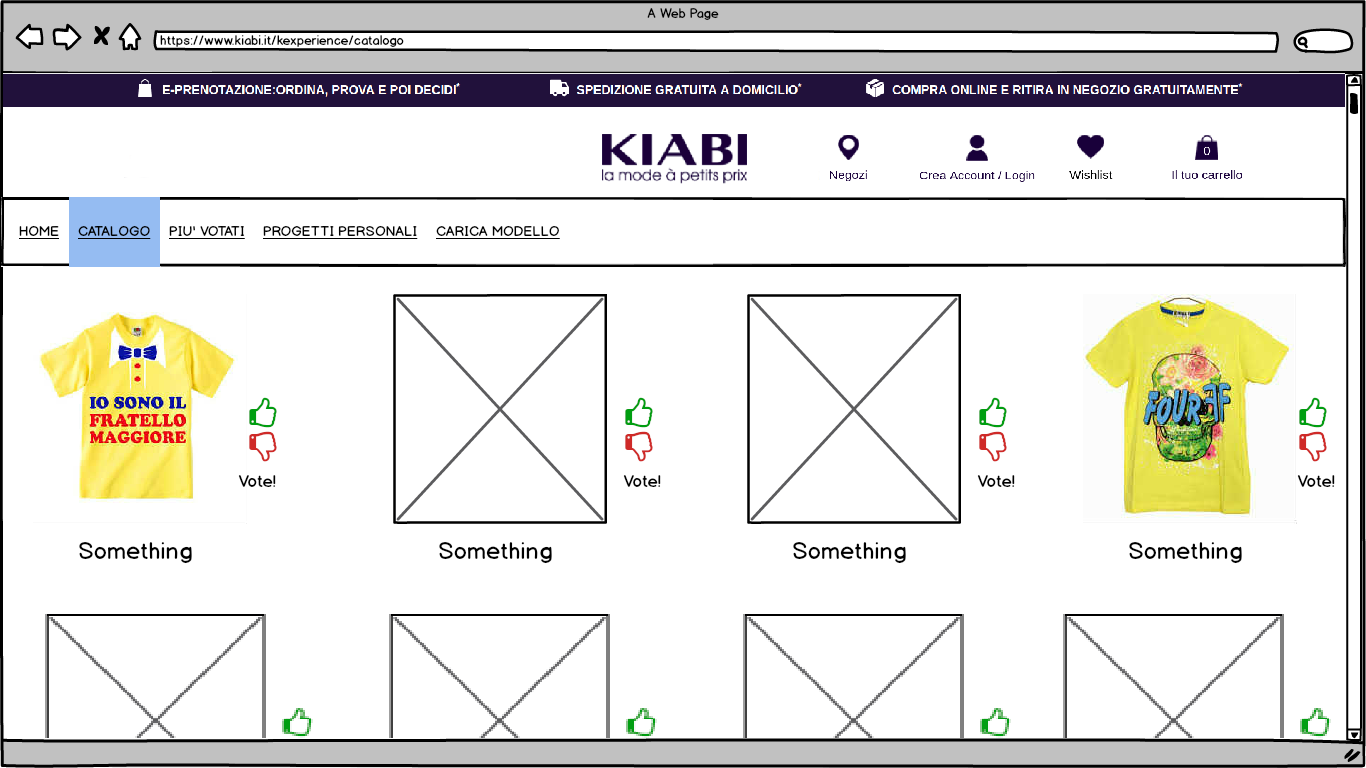
\includegraphics{img/balsamiq/Catalogo.png}
\caption{Catalogo}
\end{figure}

Il catalogo è una delle sezioni principali e contine al suo interno
tutte le creazioni degli utenti che hanno deciso di salvarle, ordinate
per numero di acquisti.

Premendo su una singola maglietta viene mostrato un modale riepilogativo
che contiene costo totale della maglietta, l'elenco delle
personalizzazioni applicate e l'autore.

\begin{figure}[h]
\centering
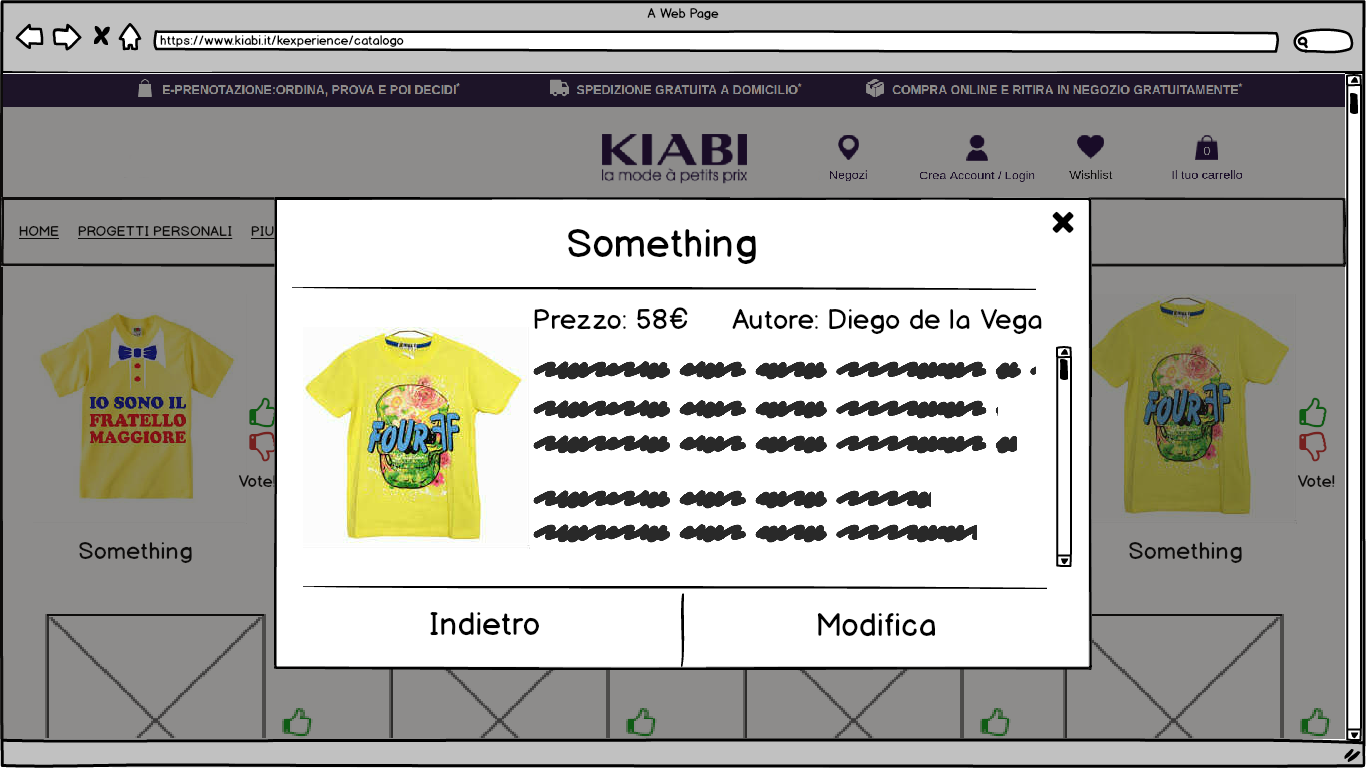
\includegraphics{img/balsamiq/Catalogodetails.png}
\caption{Catalogo - dettaglio}
\end{figure}

A fianco ad ogni immagine sono presenti due bottoni che permettono agli
utenti loggati di votare positivamente o negativamente una maglietta.
Nel caso un utente non loggato tentasse di votare, viene mostrato un
avviso che lo invita a fare login.

\begin{figure}[h]
\centering
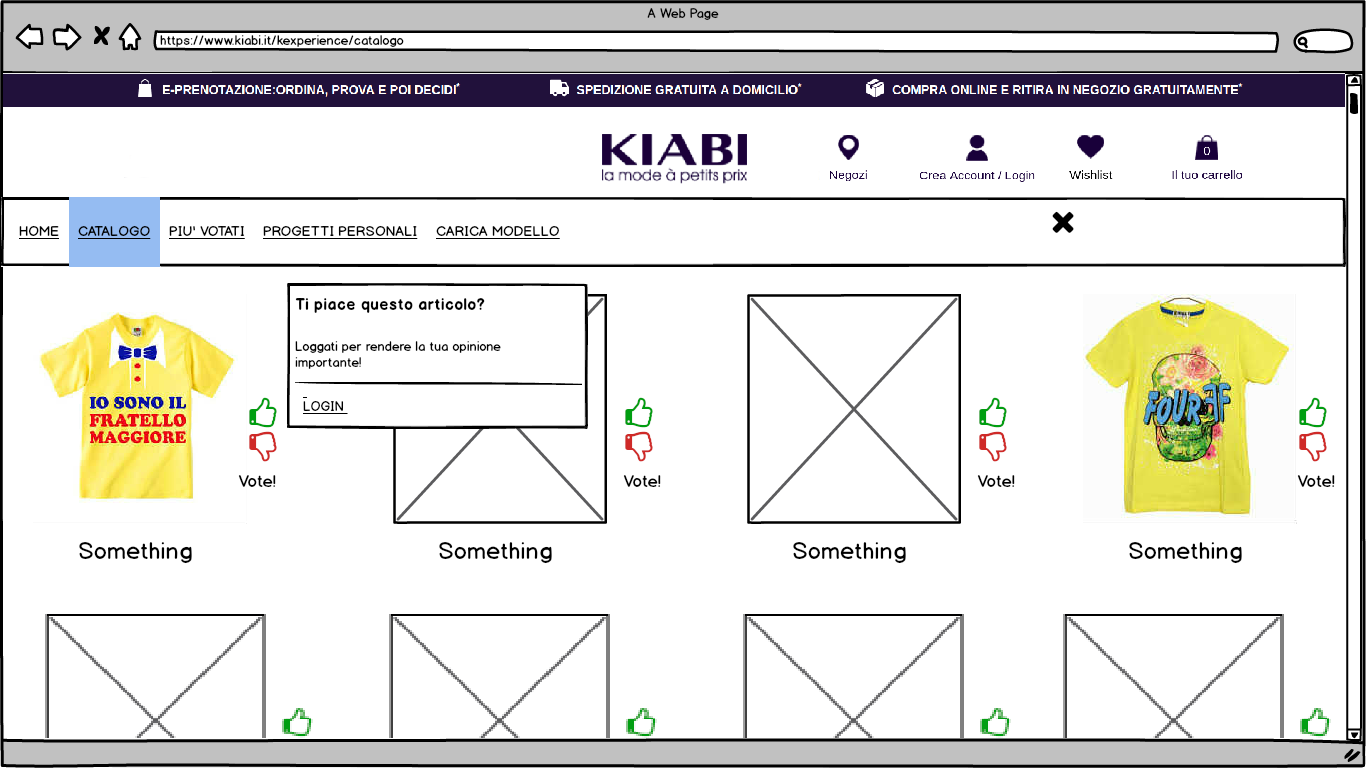
\includegraphics{img/balsamiq/Catalogologin.png}
\caption{Catalogo - login}
\end{figure}

\hypertarget{piuxf9-votati}{%
\subsection{Più votati}\label{piuxf9-votati}}

\begin{figure}[h]
\centering
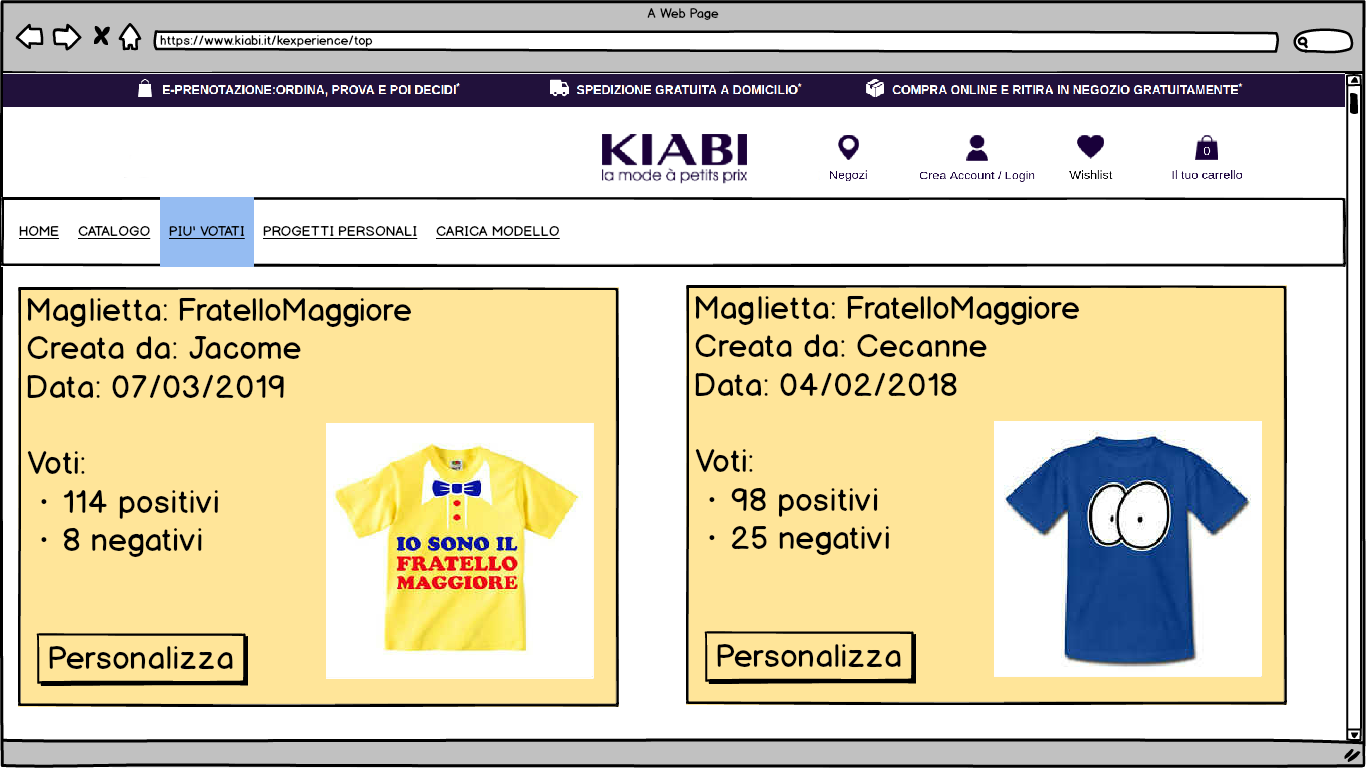
\includegraphics{img/balsamiq/MostRated.png}
\caption{Più votati}
\end{figure}

In questa pagina sono mostrate, ordinate per numero di voti, le
magliette più votate dall'utenza. Per ogni maglietta sono mostrati
l'autore, il numero di voti, la data di creazione ed un titolo per il
progetto. Premendo sul bottone personalizza si può modificare la
maglietta e procedere con l'acquisto.

\hypertarget{progetti-personali}{%
\subsection{Progetti personali}\label{progetti-personali}}

\begin{figure}[h]
\centering
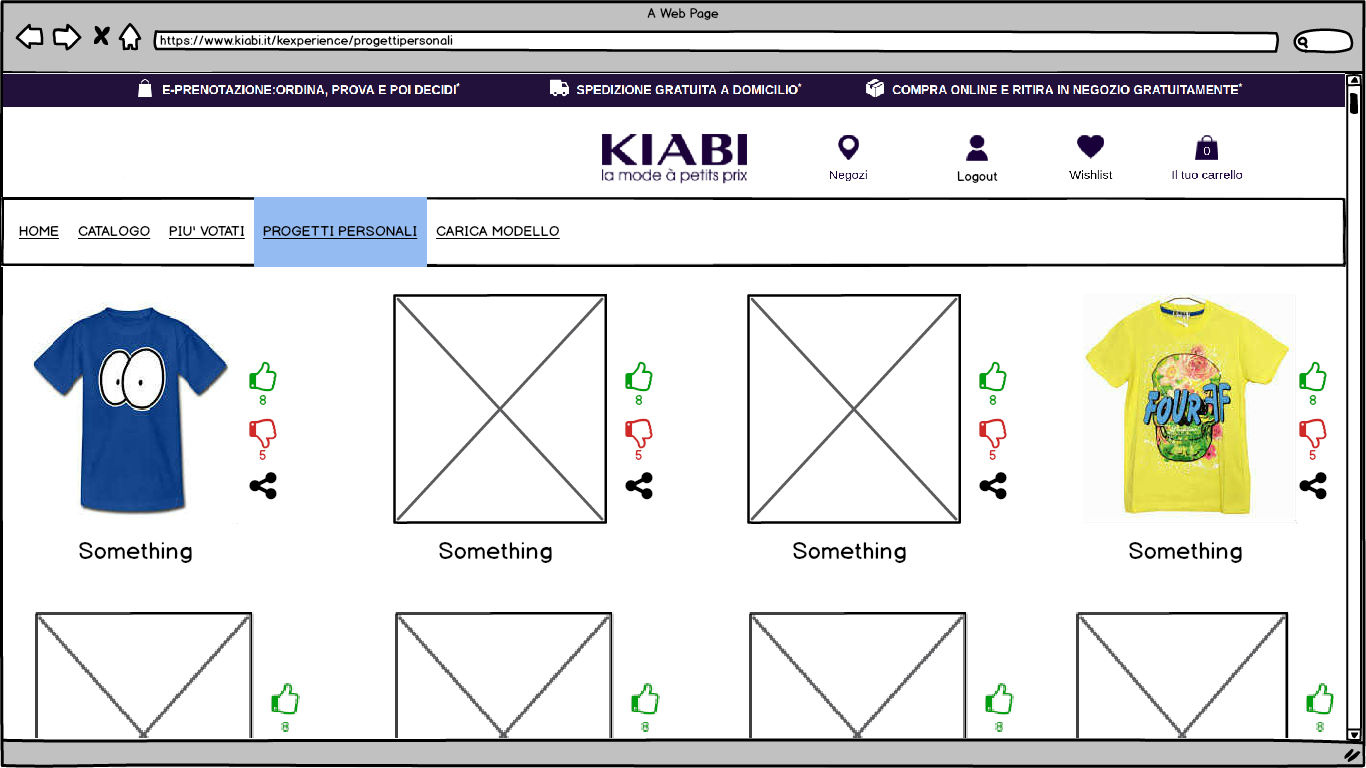
\includegraphics{img/balsamiq/ProgettiPersonali.png}
\caption{Progetti personali}
\end{figure}

In questa sezione vengono elencati i progetti salvati dall'utente. Da
qui è possibile condividere il progetto sui sociale e vedere i voti
ricevuti. Premendo sulla miniatura di un progetto si apre un modale
riepilogativo, da cui è possibile procedere alla personalizzazione.

\begin{figure}[h]
\centering
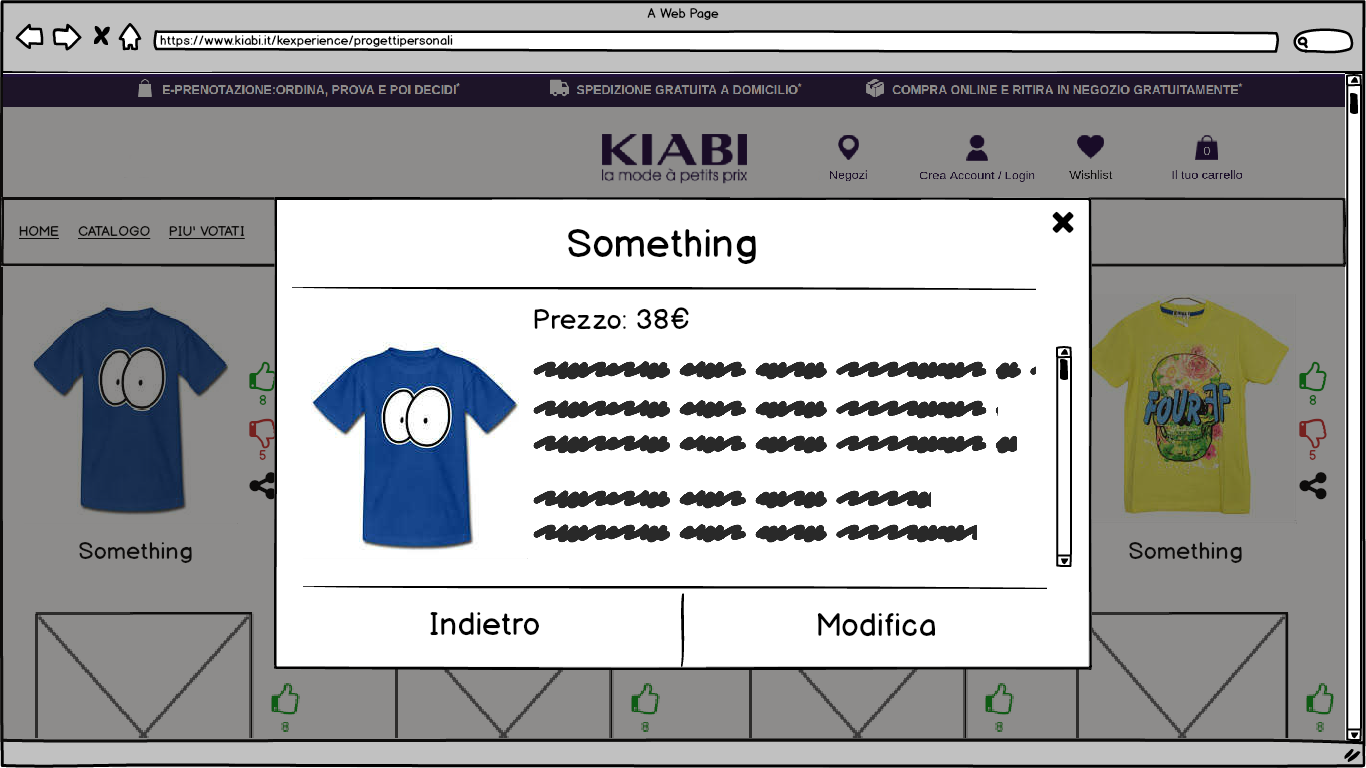
\includegraphics{img/balsamiq/ProgettiPersonalidetails.png}
\caption{Progetti personali - dettagli}
\end{figure}

\hypertarget{upload}{%
\subsection{Upload}\label{upload}}

\begin{figure}[h]
\centering
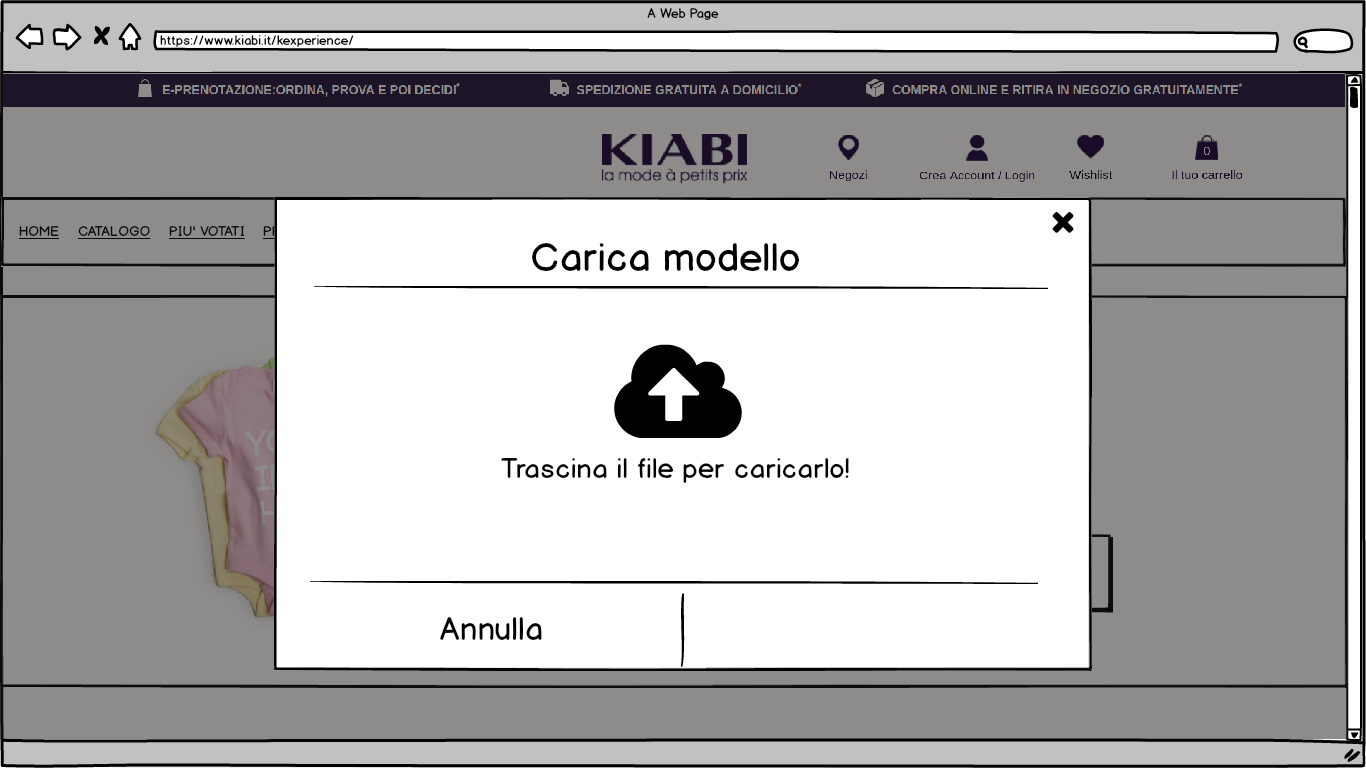
\includegraphics{img/balsamiq/UploadModel.png}
\caption{Carica modello}
\end{figure}

In ogni pagina la navbar contiene un bottone per caricare un modello,
che una volta premuto apre un modale per il caricamento. Una volta
selezionato il file da caricare, viene mostrata un'anteprima del
progetto. Da qui è possibile accedere direttamente all'editor per
continuare la personalizzazione.

\begin{figure}[h]
\centering
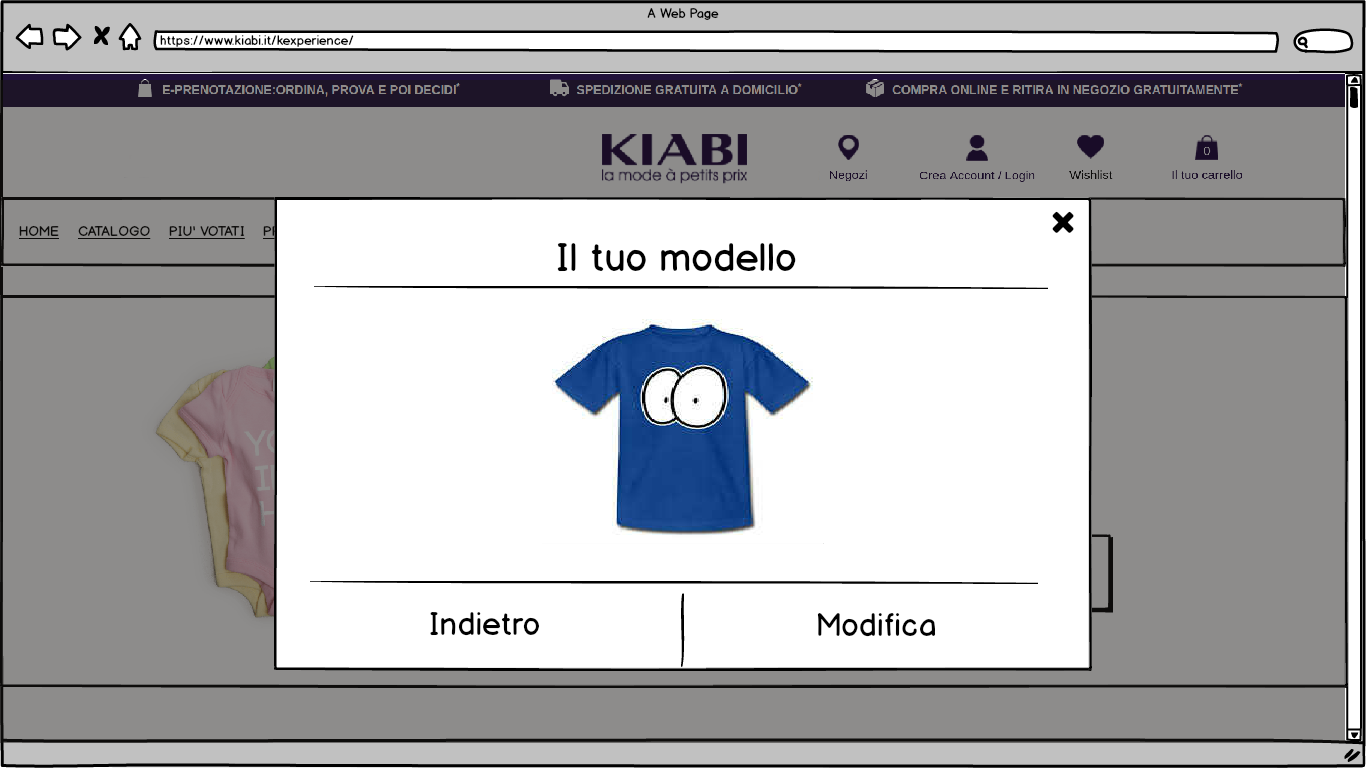
\includegraphics{img/balsamiq/UploadedModel.png}
\caption{Carica modello - anteprima}
\end{figure}

\hypertarget{valutazione-della-progettazione}{%
\chapter{Valutazione della
progettazione}\label{valutazione-della-progettazione}}

Per coerenza con l'ispezione dei sistemi esistenti si è utilizzata
un'analisi basata sulle dieci euristiche di Nielsen e Molich con
l'aggiunta di tre euristiche di Weinshenk e Barker.

\hypertarget{ispezione-err}{%
\section{Ispezione ERR}\label{ispezione-err}}

Per quanto riguarda il supporto per le task degli utenti, il prodotto è
focalizzato sulle task principali ed in particolare la creazione di una
maglietta.

È possibile visualizzare e confrontare salse ed ingredienti diversi, e
durante il processo di creazione ed acquisto l'utente è guidato in ogni
passaggio attraverso hint visuali.

Per quanto riguarda la navigazione, il sito è diviso in quattro
macroaree per l'utente non loggato, mentre l'utente loggato può visitare
un'ulteriore macroarea. ERR

\begin{longtable}[]{@{}lll@{}}
\toprule
& Utente loggato & Utente non loggato\tabularnewline
\midrule
\endhead
Homepage & X & X\tabularnewline
Editor & X & X\tabularnewline
Progetti personali & X &\tabularnewline
Catalogo & X & X\tabularnewline
Più votati & X & X\tabularnewline
\bottomrule
\end{longtable}

Le differenze tra i due tipi di utente sono il poter votare o meno un
prodotto nel catalogo e la possibilità di portare a termine un acquisto.

A livello di layout e visual design, il prodotto mantiene un insieme di
colori, icone ed elementi consistente ed offre in ogni pagina solo le
informazioni essenziali. Laddove non è chiara la relazione tra elementi,
sono presenti degli hint.

Kiabi offre già una sezione FAQ per utenti più esperti, che abbiamo
ampliato con le domande maggiormente fatte in fase di test, e un
servizio di chat con un operatore per i nuovi arrivati.

\hypertarget{test-utente}{%
\section{Test utente}\label{test-utente}}

Vista la mancanza di un team specializzato per il testing del software,
si è deciso di utilizzare il Discount Usability Testing. Questa
tipologia di testing risulta essere più formale, intuitiva, sequenziale
e a buon mercato, ma comunque utile come test formativo.

\hypertarget{protocollo-di-testing-1}{%
\subsection{Protocollo di testing}\label{protocollo-di-testing-1}}

Si è scelto di svolgere quattro test, con cinque utenti diversi, per
mantenere la consistenza con i test precedenti. I test, secondo la
metodologia discout testing​, sono stati eseguiti in maniera
sequenziale, eventualmente migliorando il design dopo ogni test.

I test sono eseguiti con il protocollo definito nel paragrafo X, usando
i wireframe del paragrafo Y.

\hypertarget{task-considerati}{%
\subsection{Task considerati}\label{task-considerati}}

I task considerati per gli utenti sono:

\begin{enumerate}
\def\labelenumi{\arabic{enumi}.}
\tightlist
\item
  Acquistare una maglietta personalizzata
\item
  Votare una maglietta personalizzata tra quelle presenti nel catalogo
\item
  Modificare un progetto tra quelli \emph{più votati}
\item
  Creare una maglietta personalizzata e salvarla
\end{enumerate}

Gli utenti scelti sono:

\begin{itemize}
\tightlist
\item
  Marco, 23 anni, ha una conoscenza del computer nella media, bravo a
  cucinare, ha due sorelle minori che adorano la cultura orientale.
\item
  Viviana, 24 anni, ha una discreta conoscenza del computer, sognatrice,
  sportiva, ha una nipote a cui piacciono le serie TV.
\item
  Antonio, 28 anni, ha una buona conoscenza del web, in particolare i
  social. È una influencer (549k followers) e frquenza un master in
  psicologia.
\item
  Lorenzo, 36 anni, livello tecnologico medio, ma con ottima conoscenza
  del mondo della moda.
\item
  Alessandro, 25 anni, conoscenza media del computer, ha un fratello
  minore. Studia lettere moderne e adora leggere fumetti.
\item
  Giorgia, 29 anni, laureata in ingegneria informatica, guarda solo i
  film d'azione e nel tempo libero adora fa da babysitter ai cuginetti,
  che adora.
\end{itemize}

Sono state scelte le seguenti metriche per la valutazione dell'usabilità
del sistema:

\begin{itemize}
\tightlist
\item
  Svolgimento: successo, fallimento
\item
  Errori: Nielsen
\item
  Efficienza: alta, media, bassa
\end{itemize}

\hypertarget{raccolta-dati}{%
\subsubsection{Raccolta dati}\label{raccolta-dati}}

\begin{longtable}[]{@{}lllll@{}}
\toprule
Marco & Task 1 & Task 2 & Task 3 & Task 4\tabularnewline
\midrule
\endhead
Svolgimento & Successo & Fallimento & Successo & Successo\tabularnewline
Errori & Errore grave & Errore catastrofico & / & Errore
cosmetico\tabularnewline
Efficienza & Media & Alta & Alta & Alta\tabularnewline
\bottomrule
\end{longtable}

Risposte questionario SUS:

\begin{longtable}[]{@{}ll@{}}
\toprule
Domanda & Risposta\tabularnewline
\midrule
\endhead
1 & 3\tabularnewline
2 & 2\tabularnewline
3 & 4\tabularnewline
4 & 1\tabularnewline
5 & 3\tabularnewline
6 & 2\tabularnewline
7 & 4\tabularnewline
8 & 2\tabularnewline
9 & 5\tabularnewline
10 & 2\tabularnewline
\bottomrule
\end{longtable}

\begin{longtable}[]{@{}lllll@{}}
\toprule
Viviana & Task 1 & Task 2 & Task 3 & Task 4\tabularnewline
\midrule
\endhead
Svolgimento & Successo & Successo & Successo & Successo\tabularnewline
Errori & Errore minore & / & / & /\tabularnewline
Efficienza & Media & Alta & Alta & Alta\tabularnewline
\bottomrule
\end{longtable}

Risposte questionario SUS:

\begin{longtable}[]{@{}ll@{}}
\toprule
Domanda & Risposta\tabularnewline
\midrule
\endhead
1 & 3\tabularnewline
2 & 2\tabularnewline
3 & 2\tabularnewline
4 & 1\tabularnewline
5 & 3\tabularnewline
6 & 2\tabularnewline
7 & 4\tabularnewline
8 & 1\tabularnewline
9 & 4\tabularnewline
10 & 1\tabularnewline
\bottomrule
\end{longtable}

\begin{longtable}[]{@{}lllll@{}}
\toprule
Antonio & Task 1 & Task 2 & Task 3 & Task 4\tabularnewline
\midrule
\endhead
Svolgimento & Successo & Successo & Successo & Successo\tabularnewline
Errori & / & / & / & /\tabularnewline
Efficienza & Alta & Alta & Alta & Alta\tabularnewline
\bottomrule
\end{longtable}

Risposte questionario SUS:

\begin{longtable}[]{@{}ll@{}}
\toprule
Domanda & Risposta\tabularnewline
\midrule
\endhead
1 & 5\tabularnewline
2 & 2\tabularnewline
3 & 5\tabularnewline
4 & 1\tabularnewline
5 & 4\tabularnewline
6 & 1\tabularnewline
7 & 3\tabularnewline
8 & 1\tabularnewline
9 & 4\tabularnewline
10 & 1\tabularnewline
\bottomrule
\end{longtable}

\begin{longtable}[]{@{}lllll@{}}
\toprule
Lorenzo & Task 1 & Task 2 & Task 3 & Task 4\tabularnewline
\midrule
\endhead
Svolgimento & Successo & Successo & Successo & Successo\tabularnewline
Errori & Errore minore & / & / & /\tabularnewline
Efficienza & Media & Alta & Alta & Alta\tabularnewline
\bottomrule
\end{longtable}

Risposte questionario SUS:

\begin{longtable}[]{@{}ll@{}}
\toprule
Domanda & Risposta\tabularnewline
\midrule
\endhead
1 & 4\tabularnewline
2 & 4\tabularnewline
3 & 5\tabularnewline
4 & 2\tabularnewline
5 & 3\tabularnewline
6 & 3\tabularnewline
7 & 4\tabularnewline
8 & 2\tabularnewline
9 & 3\tabularnewline
10 & 1\tabularnewline
\bottomrule
\end{longtable}

\begin{longtable}[]{@{}lllll@{}}
\toprule
Alessandro & Task 1 & Task 2 & Task 3 & Task 4\tabularnewline
\midrule
\endhead
Svolgimento & Successo & Successo & Successo & Successo\tabularnewline
Errori & Errore grave, cosmetico & Errore minore & / & /\tabularnewline
Efficienza & Bassa & Media & Alta & Alta\tabularnewline
\bottomrule
\end{longtable}

\begin{longtable}[]{@{}ll@{}}
\toprule
Domanda & Risposta\tabularnewline
\midrule
\endhead
1 & 4\tabularnewline
2 & 3\tabularnewline
3 & 4\tabularnewline
4 & 1\tabularnewline
5 & 5\tabularnewline
6 & 2\tabularnewline
7 & 4\tabularnewline
8 & 2\tabularnewline
9 & 4\tabularnewline
10 & 1\tabularnewline
\bottomrule
\end{longtable}

\begin{longtable}[]{@{}lllll@{}}
\toprule
Giorgia & Task 1 & Task 2 & Task 3 & Task 4\tabularnewline
\midrule
\endhead
Svolgimento & Successo & Successo & Successo & Successo\tabularnewline
Errori & Errore cosmetico & / & / & /\tabularnewline
Efficienza & Alta & Alta & Alta & Alta\tabularnewline
\bottomrule
\end{longtable}

\begin{longtable}[]{@{}ll@{}}
\toprule
Domanda & Risposta\tabularnewline
\midrule
\endhead
1 & 4\tabularnewline
2 & 1\tabularnewline
3 & 5\tabularnewline
4 & 1\tabularnewline
5 & 4\tabularnewline
6 & 2\tabularnewline
7 & 4\tabularnewline
8 & 1\tabularnewline
9 & 5\tabularnewline
10 & 1\tabularnewline
\bottomrule
\end{longtable}

\hypertarget{punteggi-questionario-sus}{%
\subsubsection{Punteggi questionario
SUS}\label{punteggi-questionario-sus}}

Al termine di ogni test è stato proposto ad ogni utente un questionario
di soddisfazione composto da dieci affermazioni. Le risposte sono state
date utilizzando la \emph{Scala di Likert} con valori compresi tra 1 e
5, dove 1 significa essere completamente in disaccordo con
l'affermazione data, mentre 5 essere completamente d'accordo. Il
risultato ottenuto, compreso in una scala che va da 0 a 100, è
nettamente più alto rispetto a quello ottenuto dai sitemi esistenti.

\begin{longtable}[]{@{}lllllllllllll@{}}
\caption{Riepilogo risposte SUS}\tabularnewline
\toprule
& 1 & 2 & 3 & 4 & 5 & 6 & 7 & 8 & 9 & 10 & Somma & Totale\tabularnewline
\midrule
\endfirsthead
\toprule
& 1 & 2 & 3 & 4 & 5 & 6 & 7 & 8 & 9 & 10 & Somma & Totale\tabularnewline
\midrule
\endhead
Marco & 3 & 2 & 4 & 1 & 3 & 2 & 4 & 2 & 5 & 2 & 30 & 75\tabularnewline
Viviana & 3 & 2 & 2 & 1 & 3 & 2 & 4 & 1 & 4 & 1 & 29 &
72,5\tabularnewline
Antonio & 5 & 2 & 5 & 1 & 4 & 1 & 3 & 1 & 4 & 1 & 35 &
87,5\tabularnewline
Lorenzo & 4 & 4 & 5 & 2 & 3 & 3 & 4 & 2 & 3 & 1 & 27 &
67,5\tabularnewline
Alessandro & 4 & 3 & 4 & 1 & 5 & 2 & 4 & 2 & 4 & 1 & 32 &
80\tabularnewline
Giorgia & 4 & 1 & 5 & 1 & 4 & 2 & 4 & 1 & 5 & 1 & 36 & 90\tabularnewline
\bottomrule
\end{longtable}

Nell'elenco di seguito vengono evidenziati gli errori commessi dagli
utenti nell'utilizzo di Kids Experience. Ad ogni errore verrà attribuito
un codice per identificarlo nei grafici seguenti.

\begin{itemize}
\tightlist
\item
  I link ``bambino'' e ``bambina'' presenti nella navbar della homepage
  di Kiabi venivano spesso scelti come link di accesso a Kids Experience
  (\textbf{E1})
\item
  Spesso gli utenti premevano il bottone per il salvataggio di una
  maglietta invece che acquistarla nel task 1 (\textbf{E2})
\item
  Il tasto indietro nella scheda di personalizzazione non sempre veniva
  riconosciuto (\textbf{E3})
\item
  Il tasto chiudi ((\times)) nella scheda di personalizzazione non
  sempre veniva vista (\textbf{E4})
\item
  Alcuni utenti hanno evidenziato una ridondanza nei path per le
  personalizzazioni dell'editor (\textbf{E5})
\item
  Alcuni utenti hanno notato delle inconsistenze nella lingua di alcuni
  link (\textbf{E6})
\item
  Non tutti hanno avuto subito chiaro che le modifiche fossero mostrate
  in tempo reale (\textbf{E7})
\end{itemize}

La seguente tabella classifica gli errori riscontrati in base
all'impatto, utilizzando la classificazione proposta da Nielsen.

\begin{longtable}[]{@{}llllll@{}}
\toprule
Errore & Implementativo & Catastrofico & Grave & Minore &
Cosmetico\tabularnewline
\midrule
\endhead
E1 & & & X & &\tabularnewline
E2 & & X & & &\tabularnewline
E3 & & & & X & X\tabularnewline
E4 & & & & X & X\tabularnewline
E5 & & & & & X\tabularnewline
E6 & & & & & X\tabularnewline
E7 & & & X & &\tabularnewline
\bottomrule
\end{longtable}

\hypertarget{curve-durgenza}{%
\subsubsection{Curve d'urgenza}\label{curve-durgenza}}

La curva d'urgenza è un grafico bidimensionale ``impatto vs frequenza''
in cui sono presenti i vari errori riscontrati.

\begin{figure}[h]
\centering
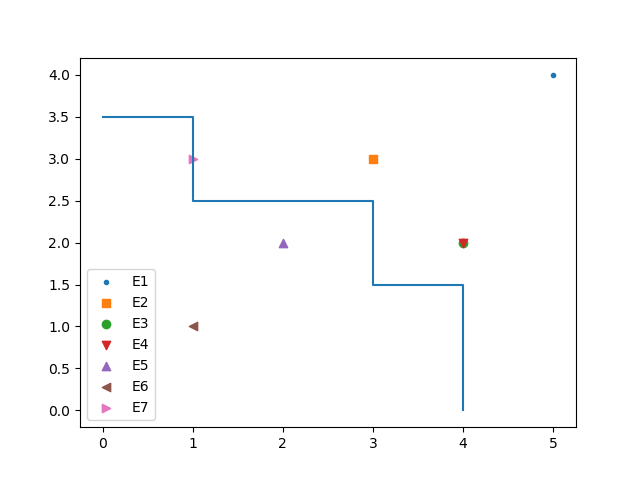
\includegraphics{img/curva_urgenza.png}
\caption{Curve d'urgenza}
\end{figure}

\hypertarget{conclusione}{%
\chapter{Conclusione}\label{conclusione}}

Visti i risultati ottenuti nei questionari SUS possiamo con certezza
affermare che il sito ha un'alta \emph{Learnability} ed una
\emph{Usability} media.

\hypertarget{licenza}{%
\chapter{Licenza}\label{licenza}}

\includegraphics{img/https://i.creativecommons.org/l/by-nc-sa/4.0/88x31.png}

Quest'opera è rilasciata sotto una licenza
\href{https://creativecommons.org/licenses/by-nc-sa/4.0/}{Creative
Commons Attribution-NonCommercial-ShareAlike 4.0 International License}.

\hypertarget{riferimenti}{%
\chapter*{Riferimenti}\label{riferimenti}}
\addcontentsline{toc}{chapter}{Riferimenti}

\hypertarget{refs}{}
\leavevmode\hypertarget{ref-eshirt}{}%
«Eshirt». s.d.
\url{https://www.eshirt.it/carrello/gt_obj_move.php?obj=0}.

\leavevmode\hypertarget{ref-redditomedio}{}%
«Il sole 24 ore: stipendi d'Italia». s.d.
\url{https://www.ilsole24ore.com/art/stipendi-d-italia-ecco-retribuzioni-nord-sud-milano-testa-vibo-valentia-coda-AE09l96E}.

\end{document}
